% =============================================================================
%  Machine Learning for Petroleum Engineers Using Python
%  Módulo 7 · Clase 1: Lo Que Antes Necesitaba un Programador
%  SLB Ecuador | UDLA
%
%  Compilar: pdflatex -shell-escape presentacion.tex (x2 para refs)
% =============================================================================
\documentclass[aspectratio=169, 11pt]{beamer}

% ── Codificación y lenguaje ──────────────────────────────────────────────────
\usepackage[T1]{fontenc}
\usepackage[utf8]{inputenc}
\usepackage[spanish,es-noshorthands]{babel}

% ── Fuentes ──────────────────────────────────────────────────────────────────
\usepackage{FiraSans}
\usepackage{FiraMono}
\renewcommand{\familydefault}{\sfdefault}

% ── Gráficos y diagramas ────────────────────────────────────────────────────
\usepackage{graphicx}
\usepackage{tikz}
\usetikzlibrary{arrows.meta, positioning, shapes.geometric, calc, fit, decorations.pathreplacing}
\usepackage{fontawesome5}

% ── Código fuente ────────────────────────────────────────────────────────────
\usepackage{minted}
\usepackage{tcolorbox}
\tcbuselibrary{minted, skins, breakable}

% ── Tablas y utilidades ──────────────────────────────────────────────────────
\usepackage{amsmath}
\usepackage{colortbl}
\usepackage{booktabs}
\usepackage{multicol}
\usepackage{hyperref}
\usepackage{calc}

% =============================================================================
%  PALETA DE COLORES (rojo UDLA + variantes)
% =============================================================================
\definecolor{arcaRed}{HTML}{C82B40}
\definecolor{arcaDark}{HTML}{6B1525}
\definecolor{udlaCrimson}{HTML}{A31545}
\definecolor{arcaGray}{HTML}{F5F5F5}
\definecolor{arcaLightGray}{HTML}{EBEBEB}
\definecolor{textDark}{HTML}{2D2D2D}
\definecolor{textMuted}{HTML}{6B7280}
\definecolor{codeGreen}{HTML}{16A34A}
\definecolor{codeBlue}{HTML}{2563EB}
\definecolor{codeOrange}{HTML}{EA580C}
\definecolor{slbBlue}{HTML}{0014DC}
\definecolor{terminalBg}{HTML}{0F172A}
\definecolor{terminalGreen}{HTML}{86EFAC}
\definecolor{terminalMuted}{HTML}{94A3B8}
\definecolor{codeBg}{HTML}{FAFAFA}

% =============================================================================
%  CONFIGURACIÓN DEL TEMA BEAMER
% =============================================================================
\usetheme{default}
\usecolortheme{default}

\setbeamertemplate{navigation symbols}{}
\setbeamertemplate{footline}{}
\setbeamertemplate{headline}{}

\setbeamercolor{normal text}{fg=textDark}
\setbeamercolor{frametitle}{fg=arcaRed, bg=white}
\setbeamercolor{title}{fg=white}
\setbeamercolor{subtitle}{fg=white!85}
\setbeamercolor{author}{fg=white!80}
\setbeamercolor{date}{fg=white!70}
\setbeamercolor{item}{fg=arcaRed}
\setbeamercolor{subitem}{fg=arcaDark}
\setbeamercolor{block title}{fg=white, bg=arcaRed}
\setbeamercolor{block body}{fg=textDark, bg=arcaGray}
\setbeamercolor{block title alerted}{fg=white, bg=codeOrange}
\setbeamercolor{block body alerted}{fg=textDark, bg=arcaGray}
\setbeamercolor{block title example}{fg=white, bg=codeGreen}
\setbeamercolor{block body example}{fg=textDark, bg=arcaGray}
\setbeamercolor{section in toc}{fg=arcaDark}

\setbeamerfont{frametitle}{size=\Large, series=\bfseries}
\setbeamerfont{title}{size=\huge, series=\bfseries}
\setbeamerfont{subtitle}{size=\large}
\setbeamerfont{author}{size=\normalsize}
\setbeamerfont{date}{size=\small}
\setbeamerfont{block title}{size=\normalsize, series=\bfseries}
\setbeamerfont{footnote}{size=\tiny}

\setbeamertemplate{itemize item}{\scriptsize\raise1.5pt\hbox{\color{arcaRed}$\blacktriangleright$}}
\setbeamertemplate{itemize subitem}{\scriptsize\raise1pt\hbox{\color{arcaDark}$\bullet$}}
\setbeamertemplate{enumerate items}[default]
\setbeamercolor{enumerate item}{fg=arcaRed}

% =============================================================================
%  HEADER
% =============================================================================
\setbeamertemplate{headline}{%
  \begin{tikzpicture}[remember picture, overlay]
    \fill[arcaDark] (current page.north west) rectangle
      ([yshift=-0.7cm]current page.north east);
    \node[anchor=west, inner sep=0pt] at
      ([xshift=0.6cm, yshift=-0.35cm]current page.north west)
      {
\includegraphics[height=0.45cm]{../logo_udla_white.png}};
    \node[anchor=east, inner sep=0pt] at
      ([xshift=-0.6cm, yshift=-0.35cm]current page.north east)
      {
\includegraphics[height=0.42cm]{../SLB_white.png}};
  \end{tikzpicture}%
  \vspace{0.7cm}%
}

% =============================================================================
%  FOOTER
% =============================================================================
\setbeamertemplate{footline}{%
  \begin{tikzpicture}[remember picture, overlay]
    \draw[arcaLightGray, line width=0.4pt]
      ([yshift=0.55cm, xshift=0.6cm]current page.south west) --
      ([yshift=0.55cm, xshift=-0.6cm]current page.south east);
    \node[anchor=south, font=\tiny\color{textMuted}] at
      ([yshift=0.15cm]current page.south)
      {Machine Learning for Petroleum Engineers Using Python \(\cdot\) SLB Ecuador};
    \node[anchor=south east, font=\scriptsize\bfseries\color{arcaRed}] at
      ([xshift=-0.6cm, yshift=0.15cm]current page.south east)
      {\insertframenumber};
  \end{tikzpicture}%
}

% =============================================================================
%  FRAMETITLE personalizado con línea roja
% =============================================================================
\setbeamertemplate{frametitle}{%
  \vspace{0.25cm}%
  \usebeamerfont{frametitle}\usebeamercolor[fg]{frametitle}\insertframetitle%
  \par\vspace{2pt}%
  \begin{tikzpicture}
    \fill[arcaRed] (0,0) rectangle (3cm, 1.5pt);
    \fill[arcaLightGray] (3cm,0) rectangle (\textwidth, 0.5pt);
  \end{tikzpicture}%
  \vspace{0.1cm}%
}

% =============================================================================
%  ESTILO DE BLOQUES DE CÓDIGO (minted + tcolorbox)
% =============================================================================
\newtcblisting{pyblock}[1][]{%
  listing engine=minted,
  minted language=python,
  minted style=xcode,
  minted options={
    fontsize=\small,
    linenos=false,
    breaklines=true,
    python3=true
  },
  enhanced,
  colback=codeBg,
  colframe=arcaRed,
  left=8pt,
  right=6pt,
  top=5pt,
  bottom=5pt,
  boxrule=0pt,
  leftrule=3pt,
  arc=3pt,
  listing only,
  title={\hspace{-2pt}\faPython\hspace{5pt}Python},
  fonttitle=\scriptsize\bfseries,
  colbacktitle=arcaRed,
  coltitle=white,
  attach boxed title to top left={xshift=8pt, yshift=-7pt},
  boxed title style={
    arc=2pt, boxrule=0pt,
    top=1.5pt, bottom=1.5pt, left=6pt, right=6pt
  },
  drop fuzzy shadow=black!12,
  #1
}

\newtcblisting{outputblock}[1][]{%
  listing engine=minted,
  minted language=text,
  minted style=bw,
  minted options={
    fontsize=\small,
    breaklines=true,
    formatcom=\color{terminalGreen}
  },
  enhanced,
  colback=terminalBg,
  colframe=terminalBg,
  coltext=terminalGreen,
  left=10pt, right=6pt, top=5pt, bottom=5pt,
  boxrule=0pt,
  arc=3pt,
  listing only,
  title={\hspace{-2pt}\faTerminal\hspace{5pt}Output},
  fonttitle=\scriptsize\bfseries,
  colbacktitle=terminalGreen!85!black,
  coltitle=terminalBg,
  attach boxed title to top left={xshift=8pt, yshift=-7pt},
  boxed title style={
    arc=2pt, boxrule=0pt,
    top=1.5pt, bottom=1.5pt, left=6pt, right=6pt
  },
  #1
}

% =============================================================================
%  SECTION DIVIDERS
% =============================================================================
\newcommand{\sectionframe}[2]{%
  \begingroup
    \setbeamertemplate{headline}{}
    \setbeamertemplate{footline}{}
    \setbeamertemplate{navigation symbols}{}
    \begin{frame}[plain, noframenumbering]
      \begin{tikzpicture}[remember picture, overlay]
        \fill[arcaRed] (current page.south west) rectangle (current page.north east);
        \node[anchor=center, text=white, font=\Huge\bfseries, text width=15cm,
              align=center] at ([yshift=0.5cm]current page.center)
              {\hyphenpenalty=10000\exhyphenpenalty=10000 #1};
        \node[anchor=center, text=white!80, font=\large, text width=10cm,
              align=center] at ([yshift=-0.8cm]current page.center) {#2};
      \end{tikzpicture}
    \end{frame}
  \endgroup
}

% =============================================================================
%  METADATOS
% =============================================================================
\title{Machine Learning for Petroleum Engineers\\Using Python}
\subtitle{Módulo 7 · Clase 1: Lo Que Antes Necesitaba un Programador}
\author{Carlos Enrique Mosquera Trujillo}
\date{2026}

% =============================================================================
%  DOCUMENTO
% =============================================================================
% =============================================================================
%  DOCUMENTO
% =============================================================================
% =============================================================================
%  Bloques de PROMPT: lo que el alumno copia y pega al agente.
%  Se usa tcolorbox (no minted) para que el texto largo se ajuste solo.
% =============================================================================
\newtcolorbox{prompt}[1][]{%
  colback=arcaGray, colframe=arcaDark, boxrule=0pt, leftrule=3.5pt,
  arc=3pt, left=8pt, right=8pt, top=6pt, bottom=6pt,
  fontupper=\ttfamily\scriptsize\color{textMuted},
  title={\hspace{-2pt}\faRobot\hspace{5pt}#1},
  fonttitle=\scriptsize\bfseries\sffamily,
  colbacktitle=arcaDark, coltitle=white,
  attach boxed title to top left={xshift=8pt, yshift=-7pt},
  boxed title style={arc=2pt, boxrule=0pt,
    top=1.5pt, bottom=1.5pt, left=6pt, right=6pt}}

\begin{document}
% ── PORTADA ──────────────────────────────────────────────────────────────────
{
\setbeamertemplate{headline}{}
\setbeamertemplate{footline}{}
\begin{frame}[plain, noframenumbering]
  \begin{tikzpicture}[remember picture, overlay]
    \fill[white] (current page.south west) rectangle (current page.north east);
    \fill[arcaRed] (current page.north west) rectangle ([yshift=-0.35cm]current page.north east);
    \fill[arcaDark] (current page.south west) rectangle ([yshift=0.35cm]current page.south east);
    \fill[arcaRed]
      ([xshift=1.1cm, yshift=-0.35cm]current page.north west) rectangle
      ([xshift=1.15cm, yshift=0.35cm]current page.south west);
    \node[anchor=north west, inner sep=0pt] at
      ([xshift=1.8cm, yshift=-1.2cm]current page.north west)
      {
\includegraphics[height=1.6cm]{../logo_udla.png}};
    \node[anchor=north east, inner sep=0pt] at
      ([xshift=-1.5cm, yshift=-1.2cm]current page.north east)
      {
\includegraphics[height=1.5cm]{../SLB.png}};
    \node[anchor=center, text=arcaDark, text width=14.5cm, align=center] at
      ([yshift=0.95cm]current page.center) {
        {\LARGE\bfseries Machine Learning for Petroleum Engineers}\\[8pt]
        {\LARGE\bfseries Using Python}
      };
    \fill[arcaRed]
      ([yshift=-0.35cm, xshift=-3.2cm]current page.center) rectangle
      ([yshift=-0.28cm, xshift=3.2cm]current page.center);
    \node[anchor=center, text=arcaRed, font=\large, text width=13cm, align=center] at
      ([yshift=-1.3cm]current page.center) {
        Módulo 7 · Clase 1\\[3pt]
        Lo Que Antes Necesitaba un Programador
      };
    \node[anchor=center, text=textMuted, font=\normalsize] at
      ([yshift=-2.5cm]current page.center) {
        {\color{arcaRed}\faUser}\hspace{6pt}Carlos Enrique Mosquera Trujillo
        \hspace{16pt}
        {\color{arcaRed}\faIndustry}\hspace{4pt}SLB Ecuador
      };
  \end{tikzpicture}
\end{frame}
}

% ── DÓNDE ESTAMOS ────────────────────────────────────────────────────────────
\begin{frame}[shrink=5]{Dónde Estamos: Cambia la Pregunta}
  \vspace{-2pt}
  \begin{columns}[T]
    \begin{column}{0.48\textwidth}
      {\small\color{arcaDark}\bfseries\faCheckCircle\hspace{5pt}Hasta aquí:}
      \vspace{4pt}
      {\footnotesize\color{textMuted}
      \begin{itemize}\setlength{\itemsep}{4pt}
        \item[{\color{codeGreen}\scriptsize\faCheck}]
          Aprendieron a \textbf{plantear} un problema de datos
        \item[{\color{codeGreen}\scriptsize\faCheck}]
          A \textbf{medir} si un modelo sirve, contra un rival simple
        \item[{\color{codeGreen}\scriptsize\faCheck}]
          A \textbf{desconfiar} del dato antes que del modelo
        \item[{\color{codeGreen}\scriptsize\faCheck}]
          Y a entregar una \textbf{banda}, no un número solo
      \end{itemize}}
      \vspace{5pt}
      {\scriptsize\color{textMuted}\itshape
       Todo eso es criterio de ingeniería. No caduca.}
    \end{column}
    \begin{column}{0.48\textwidth}
      {\small\color{arcaDark}\bfseries\faForward\hspace{5pt}Desde hoy:}
      \vspace{4pt}
      {\footnotesize\color{textMuted}
      \begin{itemize}\setlength{\itemsep}{4pt}
        \item[{\color{arcaRed}\scriptsize\faArrowRight}]
          Ya no preguntamos \emph{«¿qué modelo uso?»}
        \item[{\color{arcaRed}\scriptsize\faArrowRight}]
          Preguntamos \textbf{«¿cómo construyo la herramienta que hace falta?»}
        \item[{\color{arcaRed}\scriptsize\faArrowRight}]
          Y la construimos \textbf{dirigiendo a un agente}, no escribiendo
          cada línea
        \item[{\color{arcaRed}\scriptsize\faStar}]
          Al final de hoy, cada uno tiene una \textbf{aplicación con un link}
      \end{itemize}}
    \end{column}
  \end{columns}
  \vspace{5pt}
  {\scriptsize\color{arcaDark}\itshape
   Y como siempre: nada se da por sabido. Nadie tiene que haber programado
   antes.}
\end{frame}

% ── ANDRAGOGÍA ───────────────────────────────────────────────────────────────
\begin{frame}[shrink=5]{Ustedes Ya Dirigen Trabajo Técnico}
  \vspace{-2pt}
  {\footnotesize\color{textMuted}
  Cuando le encargan un trabajo a un contratista, ya hacen exactamente lo que
  vamos a hacer hoy con un agente:}
  \vspace{7pt}
  \begin{columns}[T]
    \begin{column}{0.31\textwidth}
      \begin{tcolorbox}[colback=arcaGray, colframe=arcaDark, boxrule=0pt,
        leftrule=3pt, arc=3pt, left=6pt, right=6pt, top=5pt, bottom=5pt]
        {\scriptsize\color{arcaDark}\bfseries 1 · Especifican}\\[3pt]
        {\scriptsize\color{textMuted}
         No dicen «arregle el pozo». Dicen qué, con qué materiales, para
         cuándo y cómo se sabe que quedó bien.}
      \end{tcolorbox}
    \end{column}
    \begin{column}{0.31\textwidth}
      \begin{tcolorbox}[colback=arcaGray, colframe=arcaDark, boxrule=0pt,
        leftrule=3pt, arc=3pt, left=6pt, right=6pt, top=5pt, bottom=5pt]
        {\scriptsize\color{arcaDark}\bfseries 2 · Reciben y revisan}\\[3pt]
        {\scriptsize\color{textMuted}
         No firman el acta sin mirar. Revisan contra lo que pidieron,
         no contra lo que les entregaron.}
      \end{tcolorbox}
    \end{column}
    \begin{column}{0.31\textwidth}
      \begin{tcolorbox}[colback=arcaGray, colframe=arcaDark, boxrule=0pt,
        leftrule=3pt, arc=3pt, left=6pt, right=6pt, top=5pt, bottom=5pt]
        {\scriptsize\color{arcaDark}\bfseries 3 · Responden}\\[3pt]
        {\scriptsize\color{textMuted}
         Si el trabajo sale mal, la firma es de ustedes. El contratista no
         va a la reunión.}
      \end{tcolorbox}
    \end{column}
  \end{columns}
  \vspace{9pt}
  {\footnotesize\color{arcaDark}\itshape
   Un agente de código es un contratista muy rápido, muy barato y muy seguro
   de sí mismo. Todo lo que ya saben sobre dirigir contratistas aplica ---
   incluida la parte de que la firma sigue siendo suya.}
\end{frame}

% ═════════════════════════════════════════════════════════════════════════════
\sectionframe{Esto Ya Pasó}{Cómo se escribe código en 2026, con números \\[6pt] \normalsize 0 -- 15 min}
% ═════════════════════════════════════════════════════════════════════════════

\begin{frame}[shrink=8]{La Foto de 2026}
  \vspace{-2pt}
  \begin{center}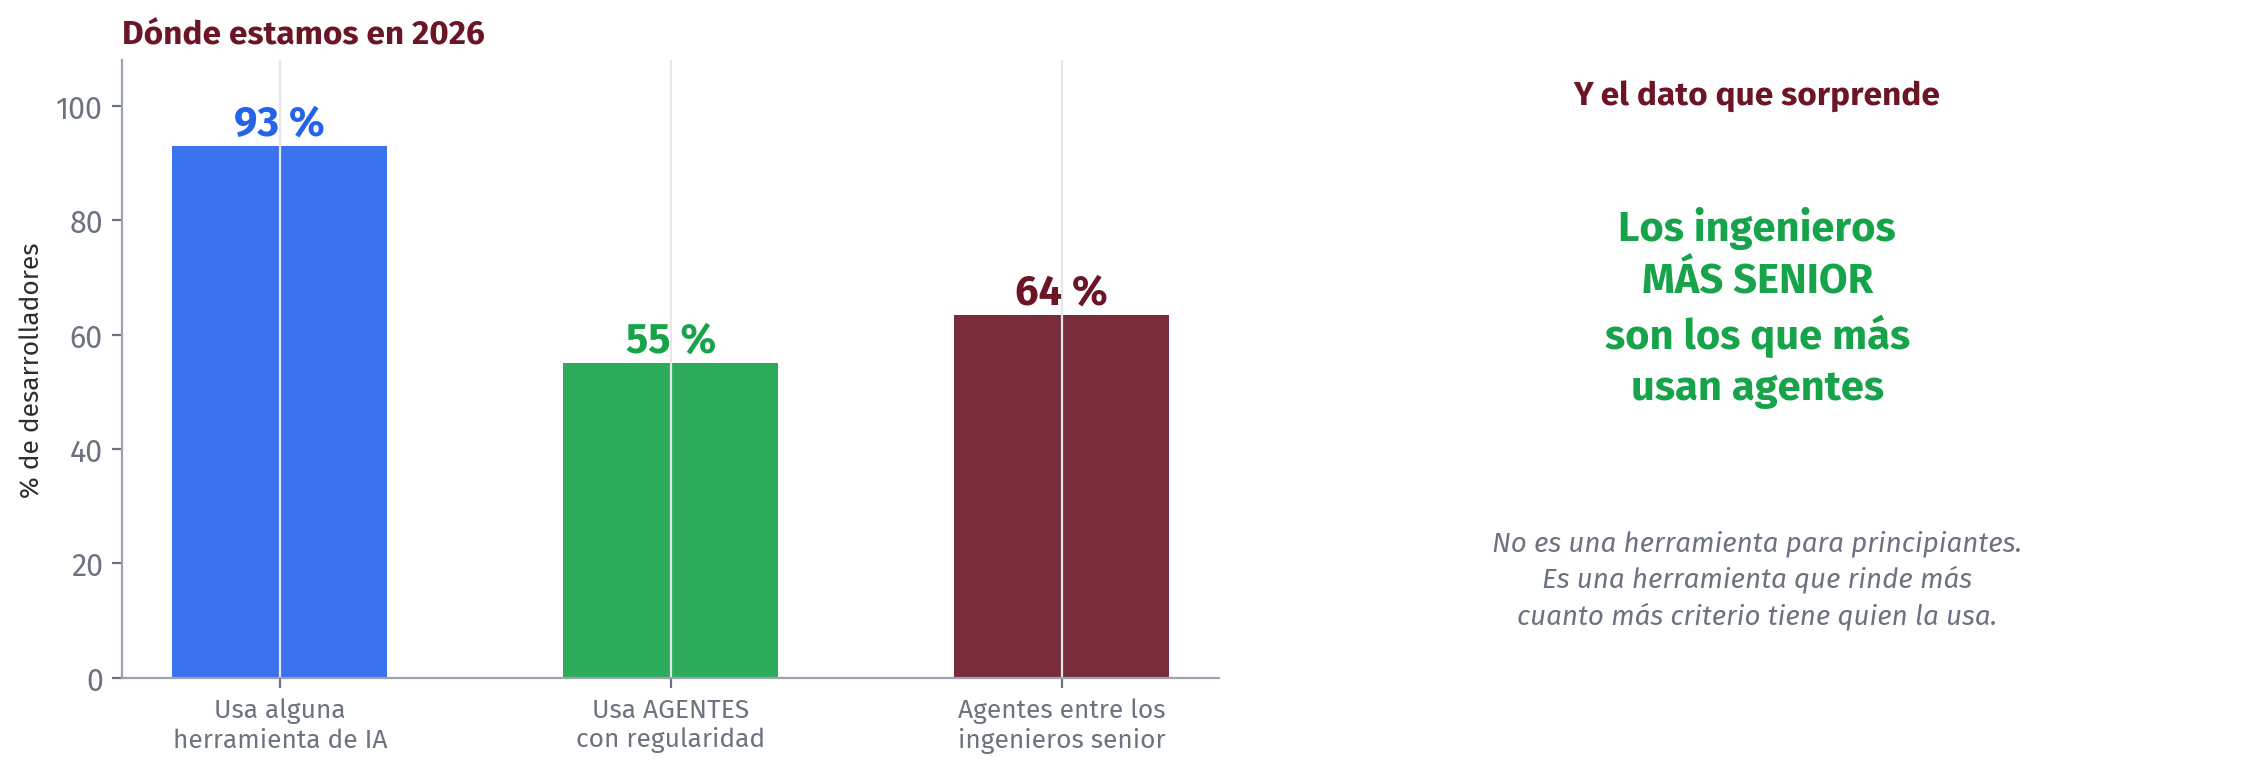
\includegraphics[width=0.95\textwidth, height=0.46\textheight, keepaspectratio]{fig_adopcion.png}\end{center}
  \vspace{2pt}
  {\footnotesize\color{textMuted}
   Esto ya no es una tendencia ni una moda: es cómo se trabaja. El
   \textbf{93\,\%} de los desarrolladores usa alguna herramienta de IA, y más
   de la mitad usa \textbf{agentes} con regularidad.}
\end{frame}

\begin{frame}[shrink=6]{El Dato que le Conviene a Esta Sala}
  \vspace{4pt}
  \begin{tcolorbox}[colback=arcaGray, colframe=codeGreen, boxrule=0pt,
    leftrule=4pt, arc=3pt, left=10pt, right=10pt, top=8pt, bottom=8pt]
    {\large\color{arcaDark}\bfseries
     Los ingenieros \textbf{más senior} son los que \textbf{más} usan
     agentes: 63,5\,\% contra 55\,\% del promedio.}
  \end{tcolorbox}
  \vspace{9pt}
  {\footnotesize\color{textMuted}
   No es una herramienta para el que no sabe. Es una herramienta que
   \textbf{rinde más cuanto más criterio tiene quien la usa} --- porque el que
   sabe reconoce al instante cuándo la respuesta está mal.
   \vspace{7pt}

   Y hay un segundo dato en la misma dirección: quien usa agentes tiene
   \textbf{el doble de probabilidad} de estar entusiasmado con ellos. Quien no
   los usa, el doble de escéptico.}
  \vspace{9pt}
  {\footnotesize\color{arcaDark}\bfseries\itshape
   El escepticismo, en esto, se cura usándolo. No leyendo sobre ello.}
\end{frame}

\begin{frame}[shrink=6]{Lo que No Dicen los Titulares}
  \vspace{2pt}
  {\footnotesize\color{textMuted}
   Todo el mundo lo usa. Pero casi nadie le cree del todo, y eso también está
   medido:}
  \vspace{3pt}
  \begin{columns}[T]
    \begin{column}{0.47\textwidth}
      \begin{tcolorbox}[colback=arcaGray, colframe=arcaRed, boxrule=0pt,
        leftrule=3pt, arc=3pt, left=8pt, right=8pt, top=4pt, bottom=4pt]
        {\scriptsize\color{arcaRed}\bfseries LA CONFIANZA}\\[4pt]
        {\footnotesize\color{textMuted}
         Solo el \textbf{3\,\%} confía plenamente en lo que produce.\\[4pt]
         El \textbf{46\,\%} desconfía de su precisión, contra un 33\,\% que
         confía.}
      \end{tcolorbox}
    \end{column}
    \begin{column}{0.47\textwidth}
      \begin{tcolorbox}[colback=arcaGray, colframe=arcaRed, boxrule=0pt,
        leftrule=3pt, arc=3pt, left=8pt, right=8pt, top=4pt, bottom=4pt]
        {\scriptsize\color{arcaRed}\bfseries LA FRUSTRACIÓN \#1}\\[4pt]
        {\footnotesize\color{textMuted}
         El \textbf{66\,\%} dice que lo que más le molesta son las
         \emph{«soluciones casi correctas, pero no del todo»}.\\[4pt]
         Y el \textbf{45\,\%} dice que depurarlas tarda \textbf{más} que
         escribir el código a mano.}
      \end{tcolorbox}
    \end{column}
  \end{columns}
  \vspace{3pt}
  {\footnotesize\color{arcaDark}\bfseries
   «Casi correcto, pero no» es el problema central de esta clase --- y es
   justo donde hace falta alguien que sepa del tema.}
\end{frame}

\begin{frame}[shrink=8]{El Cuello de Botella se Movió}
  \vspace{-2pt}
  \begin{center}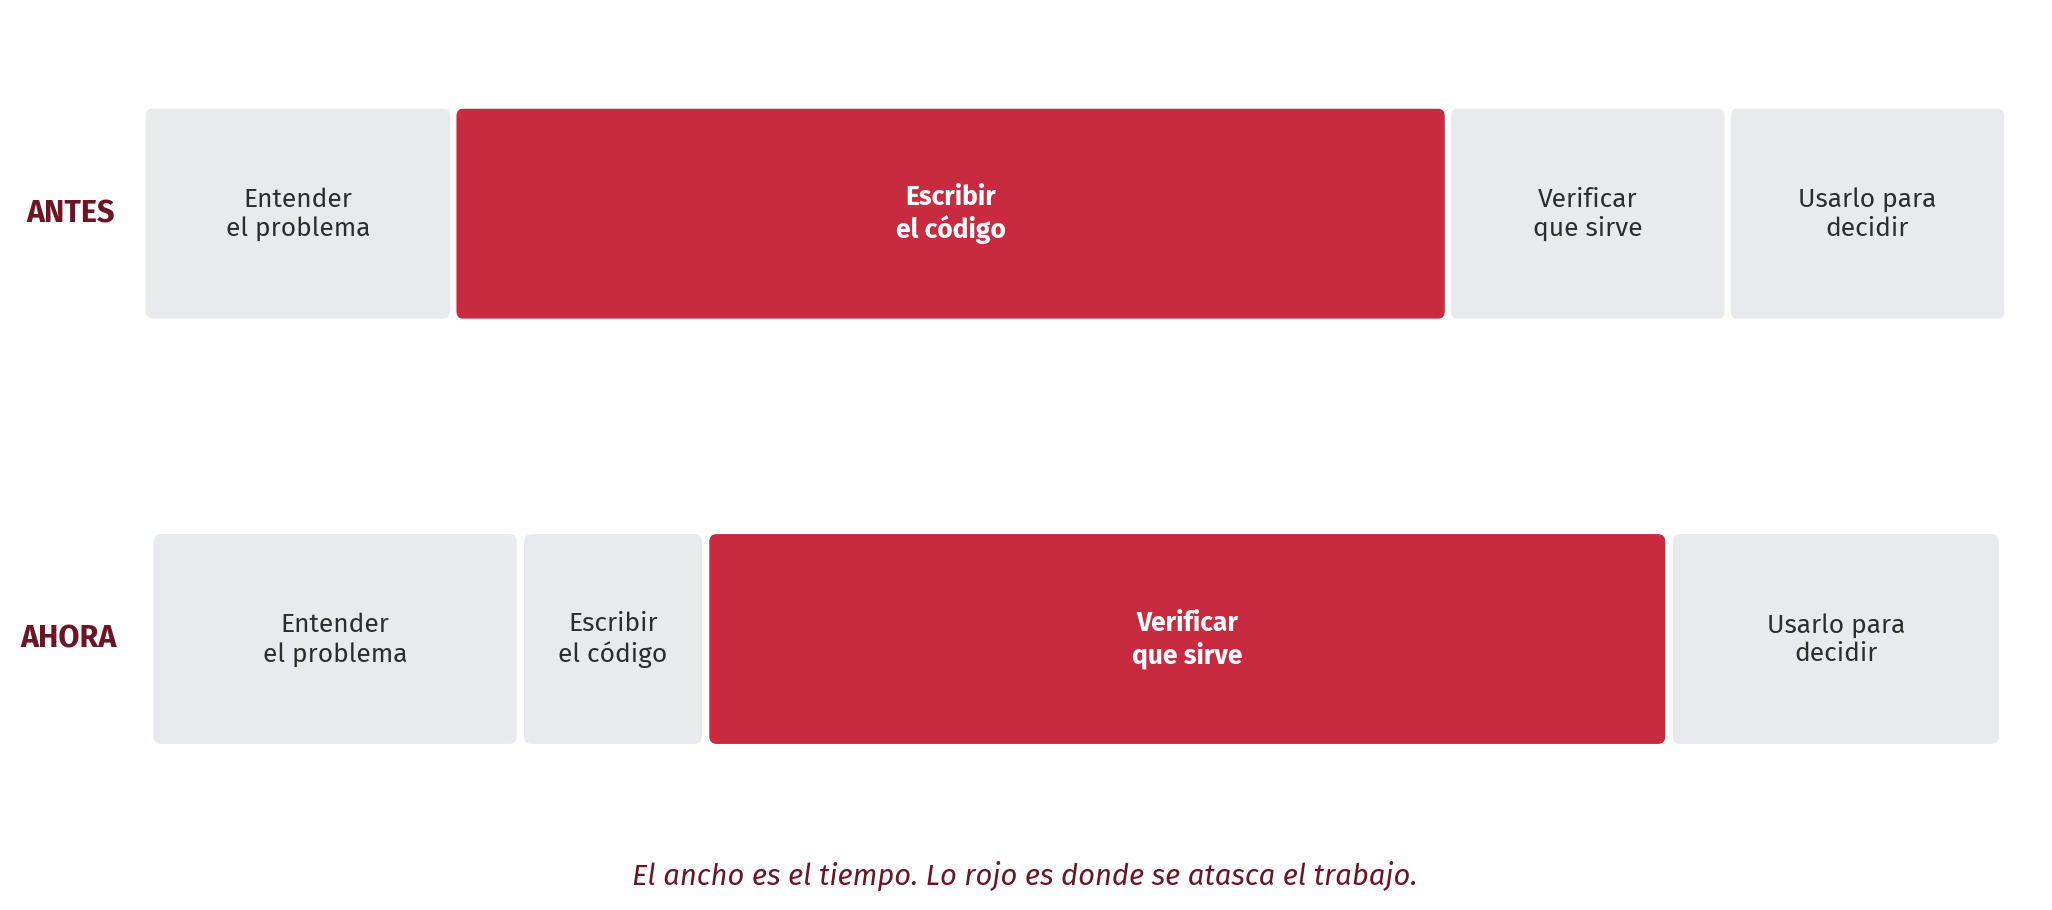
\includegraphics[width=0.90\textwidth, height=0.46\textheight, keepaspectratio]{fig_cuello_botella.png}\end{center}
  \vspace{2pt}
  {\footnotesize\color{textMuted}
   Escribir código dejó de ser lo caro. Lo caro ahora es \textbf{verificar}:
   los cambios hechos con IA esperan más tiempo en revisión, y meten más
   errores si nadie los mira.}
\end{frame}

\begin{frame}[shrink=6]{Y Por Eso Ustedes Valen Más, No Menos}
  \vspace{4pt}
  \begin{tcolorbox}[colback=arcaGray, colframe=arcaRed, boxrule=0pt,
    leftrule=4pt, arc=3pt, left=10pt, right=10pt, top=9pt, bottom=9pt]
    {\large\color{arcaDark}\bfseries
     Lo que se volvió barato es \emph{escribir}. Lo que sigue siendo escaso es
     \textbf{saber si el resultado tiene sentido}.}
  \end{tcolorbox}
  \vspace{9pt}
  {\footnotesize\color{textMuted}
   Un agente puede escribir en treinta segundos el código que ajusta una curva
   de declinación. Lo que no puede hacer es saber que ese campo tuvo un
   \emph{workover} en 2018, que el medidor estuvo descalibrado seis meses, o
   que ese pozo no debería estar en la muestra.
   \vspace{7pt}

   \textbf{Eso lo saben ustedes.} Y hasta hoy, para convertir ese
   conocimiento en una herramienta, había que esperar a que alguien de
   sistemas tuviera tiempo.}
  \vspace{8pt}
  {\footnotesize\color{arcaDark}\bfseries\itshape
   Eso es lo que se acabó. Y de eso se trata este módulo.}
\end{frame}

\begin{frame}[shrink=6]{Acotar el Problema}
  \vspace{2pt}
  \begin{columns}[T]
    \begin{column}{0.47\textwidth}
      \begin{tcolorbox}[colback=arcaGray, colframe=codeGreen, boxrule=0pt,
        leftrule=3pt, arc=3pt, left=8pt, right=8pt, top=6pt, bottom=6pt]
        {\scriptsize\color{codeGreen}\bfseries LO QUE SÍ VAMOS A HACER}\\[5pt]
        {\footnotesize\color{textMuted}
        \begin{itemize}\setlength{\itemsep}{3pt}
          \item[{\color{codeGreen}\scriptsize\faCheck}]
            Gráficas que se entienden solas
          \item[{\color{codeGreen}\scriptsize\faCheck}]
            Dirigir un agente para que las haga
          \item[{\color{codeGreen}\scriptsize\faCheck}]
            \textbf{Verificar} lo que devuelve
          \item[{\color{codeGreen}\scriptsize\faCheck}]
            Convertirlo en una app con link
        \end{itemize}}
      \end{tcolorbox}
    \end{column}
    \begin{column}{0.47\textwidth}
      \begin{tcolorbox}[colback=arcaGray, colframe=arcaRed, boxrule=0pt,
        leftrule=3pt, arc=3pt, left=8pt, right=8pt, top=6pt, bottom=6pt]
        {\scriptsize\color{arcaRed}\bfseries LO QUE NO}\\[5pt]
        {\footnotesize\color{textMuted}
        \begin{itemize}\setlength{\itemsep}{3pt}
          \item[{\color{arcaRed}\scriptsize\faTimes}]
            Convertirlos en programadores
          \item[{\color{arcaRed}\scriptsize\faTimes}]
            Enseñar a memorizar sintaxis
          \item[{\color{arcaRed}\scriptsize\faTimes}]
            Instalar nada: todo corre en Colab
          \item[{\color{arcaRed}\scriptsize\faTimes}]
            Modelos nuevos --- hoy es sobre
            \textbf{construir}, no sobre predecir
        \end{itemize}}
      \end{tcolorbox}
    \end{column}
  \end{columns}
  \vspace{8pt}
  {\footnotesize\color{arcaDark}\itshape
   Regla de la casa para hoy: si algo no lo entienden, es culpa del material,
   no de ustedes. Pregunten en el momento.}
\end{frame}

% ═════════════════════════════════════════════════════════════════════════════
\sectionframe{Primera Victoria}{Que sus datos se vean como lo que valen \\[6pt] \normalsize 15 -- 45 min}
% ═════════════════════════════════════════════════════════════════════════════

\begin{frame}[shrink=6]{Empecemos por Algo que Usan Todas las Semanas}
  \vspace{4pt}
  {\footnotesize\color{textMuted}
   Todos hacen reportes. Y todos han visto la misma escena: un gráfico
   correcto, con los números bien, que nadie entiende en la reunión --- y hay
   que explicarlo hablando.
   \vspace{8pt}

   Un gráfico que hay que explicar es un gráfico que falló.}
  \vspace{9pt}
  \begin{tcolorbox}[colback=arcaGray, colframe=arcaDark, boxrule=0pt,
    leftrule=4pt, arc=3pt, left=10pt, right=10pt, top=7pt, bottom=7pt]
    {\footnotesize\color{arcaDark}\bfseries
     Una gráfica no es un adorno del análisis: \textbf{es el argumento}.}\\[5pt]
    {\footnotesize\color{textMuted}
     Es lo único que la mayoría de la gente va a ver de todo su trabajo. El
     modelo, los datos y las tres semanas de esfuerzo llegan a la gerencia
     convertidos en una imagen.}
  \end{tcolorbox}
  \vspace{7pt}
  {\footnotesize\color{textMuted}
   Y es el mejor lugar para empezar a dirigir un agente: se ve el resultado
   de inmediato, y si está mal, se nota.}
\end{frame}

\begin{frame}[shrink=8]{Los Mismos Datos, Dos Veces}
  \vspace{-2pt}
  \begin{center}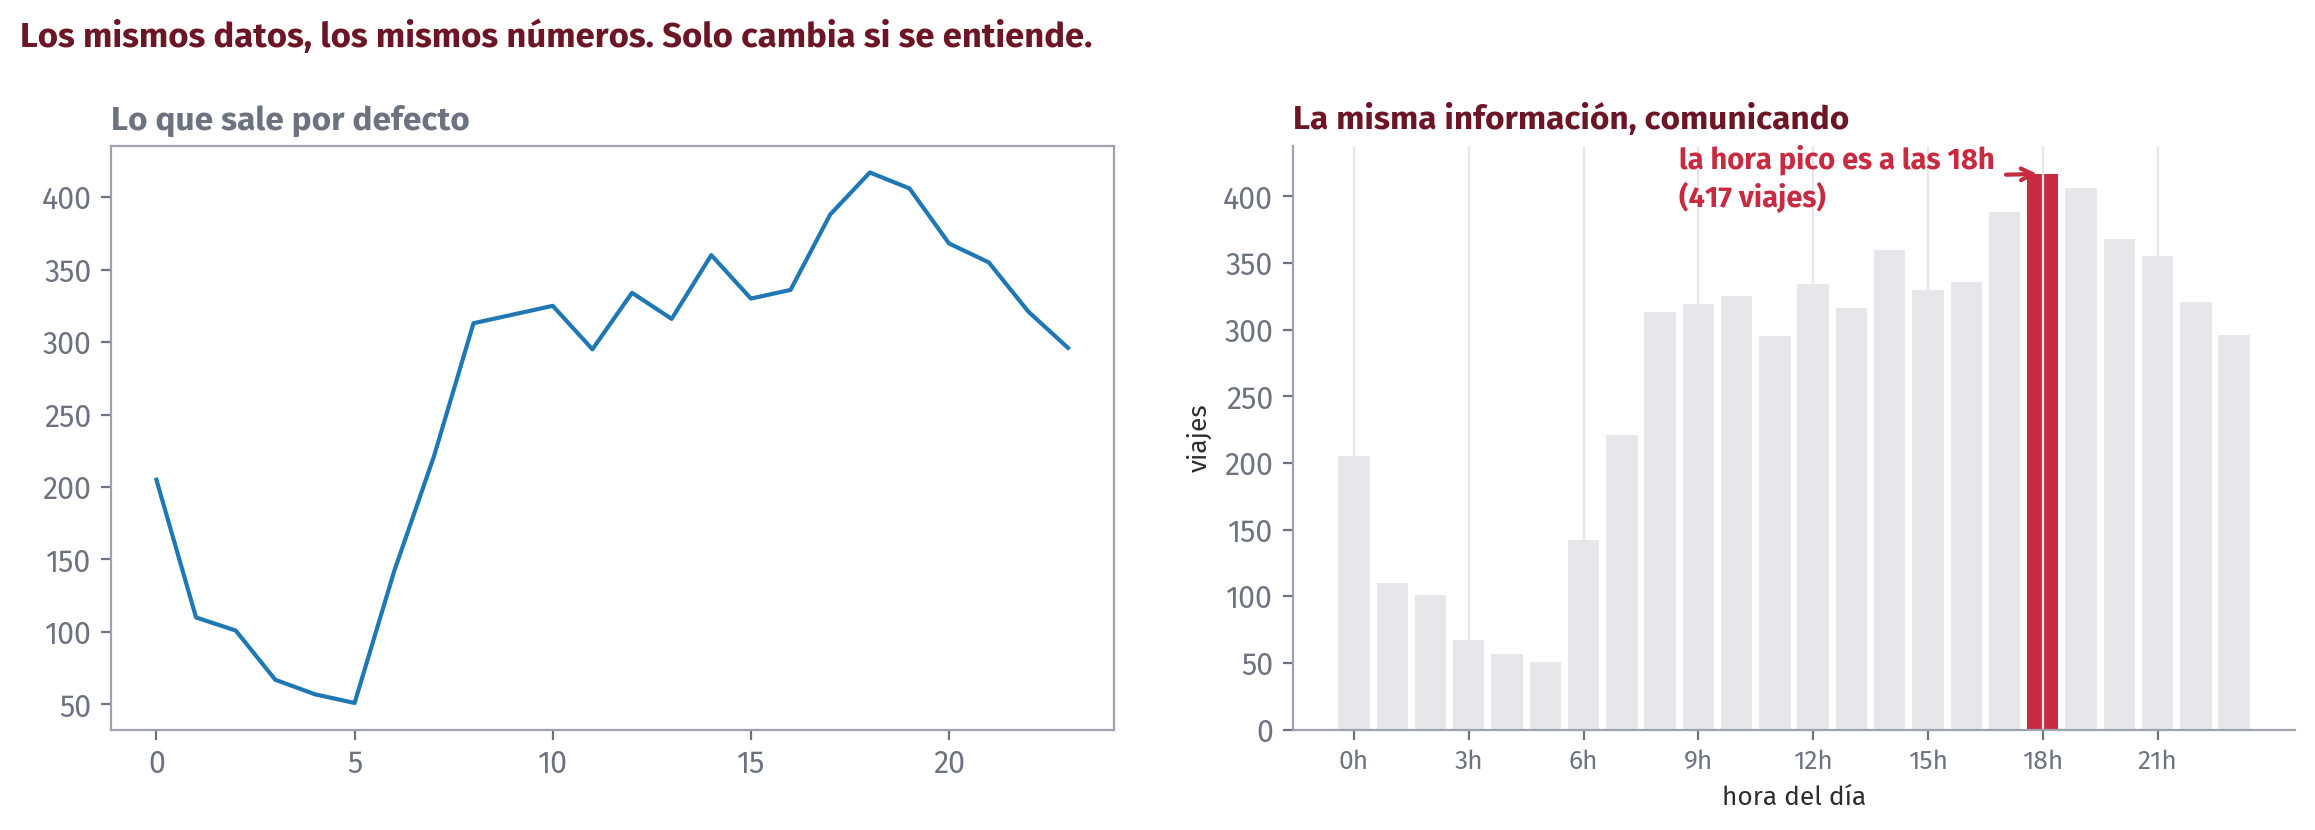
\includegraphics[width=0.97\textwidth, height=0.47\textheight, keepaspectratio]{fig_fea_vs_bonita.png}\end{center}
  \vspace{2pt}
  {\footnotesize\color{textMuted}
   Mismos datos, mismos números, misma librería. A la izquierda hay que
   explicar; a la derecha, la respuesta salta sola.}
\end{frame}

\begin{frame}[shrink=6]{Qué Cambió, Exactamente}
  \vspace{2pt}
  {\footnotesize\color{textMuted}
   No fue magia ni buen gusto. Fueron \textbf{cinco decisiones}, y todas se le
   pueden pedir a un agente:}
  \vspace{7pt}
  {\footnotesize\color{textMuted}
  \begin{enumerate}\setlength{\itemsep}{4pt}
    \item \textbf{Barras en vez de línea.} Una línea sugiere continuidad; las
          horas son categorías separadas.
    \item \textbf{Un solo color con sentido.} Gris todo, rojo lo que importa.
          El color señala, no decora.
    \item \textbf{Los ejes dicen qué son} --- «hora del día», «viajes» --- en
          el idioma del que lee.
    \item \textbf{El hallazgo, escrito sobre la figura.} Si la conclusión es
          «el pico es a las 18h», eso va en la lámina, no en la boca del
          presentador.
    \item \textbf{Se quitó todo lo demás.} Sin marco, sin cuadrícula de más,
          sin decimales que nadie necesita.
  \end{enumerate}}
  \vspace{7pt}
  {\footnotesize\color{arcaDark}\bfseries\itshape
   Ninguna de las cinco es programación. Las cinco son criterio de
   comunicación --- y por eso las tienen que decidir ustedes, no el agente.}
\end{frame}

\begin{frame}[shrink=6]{Qué Es Seaborn y Por Qué Existe}
  \vspace{4pt}
  {\footnotesize\color{textMuted}
   \textbf{Matplotlib} es la librería con la que Python dibuja. Puede hacer
   todo, pero hay que decirle todo: cada color, cada margen, cada etiqueta.
   Por eso lo que sale «por defecto» se ve así de crudo.
   \vspace{8pt}

   \textbf{Seaborn} se construyó encima. Trae decisiones de diseño ya tomadas
   por gente que estudia cómo se leen los gráficos, y entiende de tablas: uno
   le dice qué columna va en cada eje y él se encarga del resto.}
  \vspace{9pt}
  \begin{tcolorbox}[colback=arcaGray, colframe=arcaDark, boxrule=0pt,
    leftrule=3pt, arc=3pt, left=9pt, right=9pt, top=6pt, bottom=6pt]
    {\footnotesize\color{arcaDark}\bfseries
     Y ya viene instalado en Colab. No hay nada que instalar.}
  \end{tcolorbox}
  \vspace{7pt}
  {\scriptsize\color{textMuted}\itshape
   Además trae datasets de práctica listos, y de ahí salen los datos de hoy:
   una línea y ya tienen 6.433 viajes de taxi con los que trabajar.}
\end{frame}

\begin{frame}[fragile, shrink=8]{Las Tres Líneas con las que Arranca Todo}
  \vspace{2pt}
  \begin{minted}[fontsize=\small, breaklines]{python}
import seaborn as sns

taxis = sns.load_dataset("taxis")
taxis.head()
  \end{minted}
  \vspace{6pt}
  {\footnotesize\color{textMuted}
   Eso es todo. \texttt{load\_dataset} baja los datos y los deja en una tabla
   --- lo que en Python se llama un \textbf{DataFrame}: filas y columnas, como
   una hoja de cálculo, pero manejable con código.}
  \vspace{7pt}

  {\footnotesize\color{arcaDark}\bfseries
   Los datos de hoy: 6.433 viajes de taxi de Nueva York, con hora de salida y
   llegada, distancia, tarifa, propina, forma de pago y zonas.}
  \vspace{5pt}

  {\scriptsize\color{textMuted}\itshape
   ¿Por qué taxis y no pozos? Porque hoy la habilidad es lo que importa, y
   quiero que se vea que sirve igual para cualquier problema. En el proyecto
   final cada uno trae el suyo.}
\end{frame}

\begin{frame}[shrink=10]{La Misma Habilidad, Tres Problemas Distintos}
  \vspace{-2pt}
  \begin{center}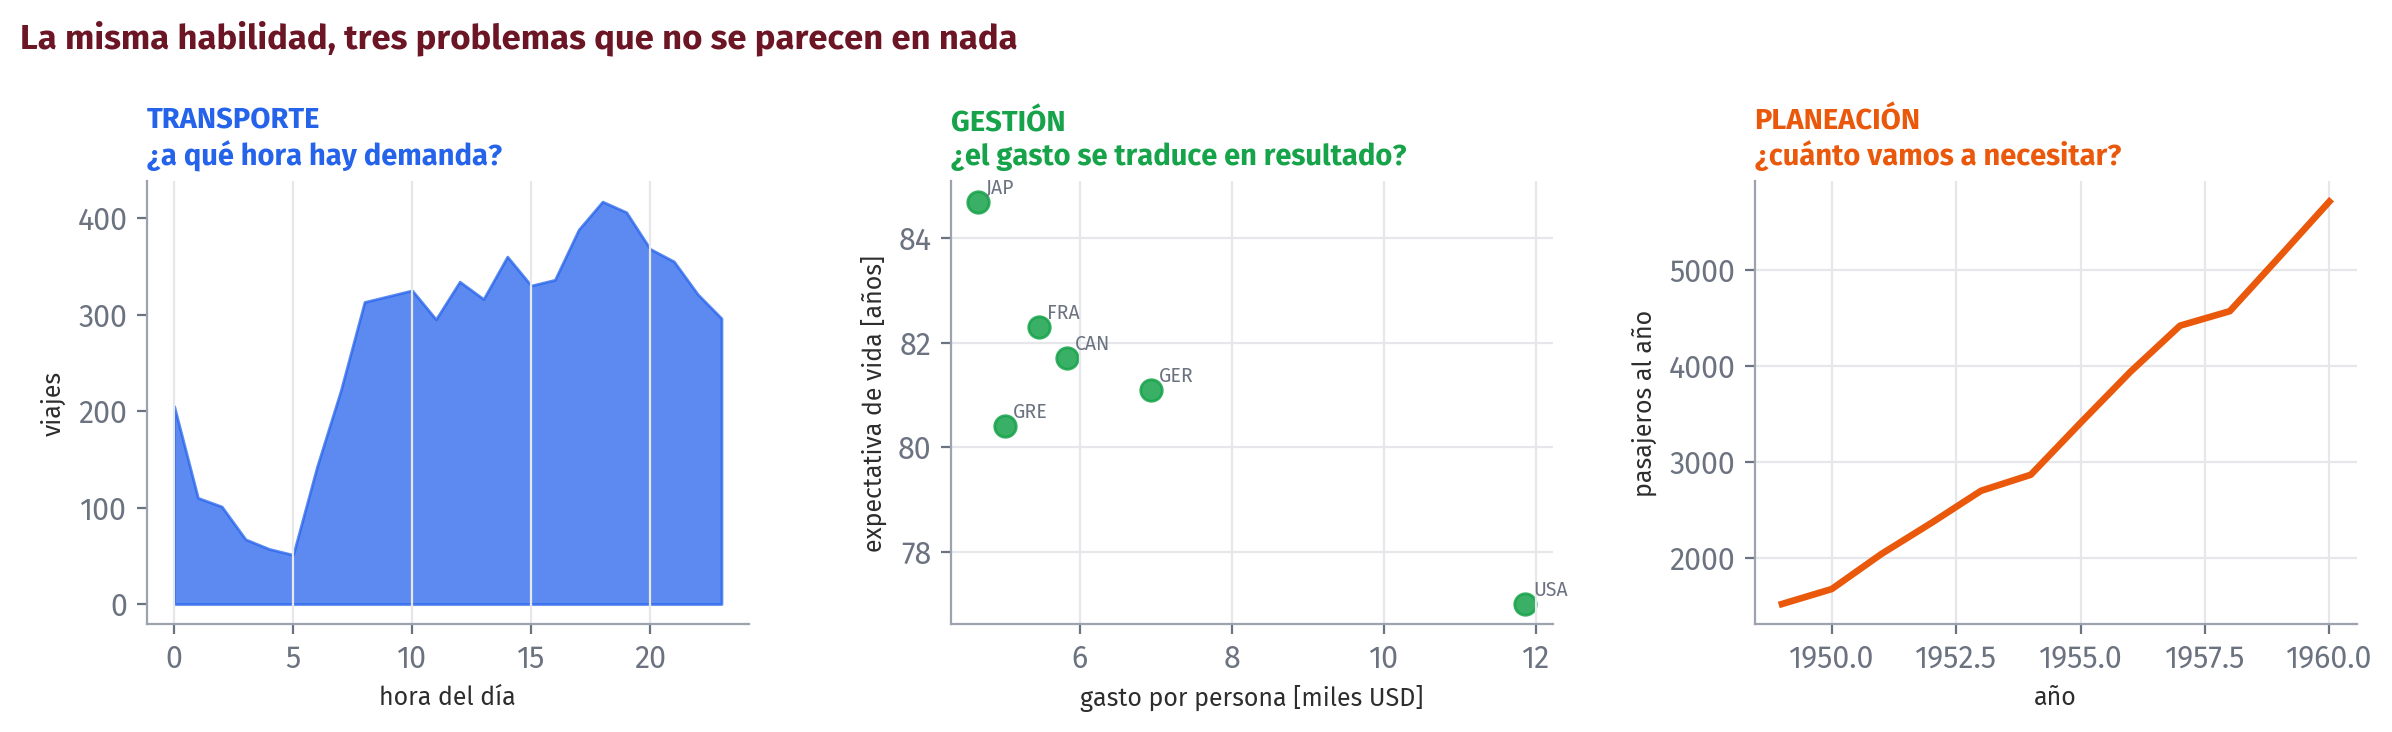
\includegraphics[width=0.97\textwidth, height=0.46\textheight, keepaspectratio]{fig_tres_dominios.png}\end{center}
  \vspace{2pt}
  {\footnotesize\color{textMuted}
   Transporte, gestión presupuestal y planeación de demanda. Tres preguntas
   que no se parecen en nada --- y la técnica para responderlas es la misma.}
\end{frame}

\begin{frame}[shrink=6]{Su Primer Encargo al Agente \hfill {\normalsize\color{arcaRed}\faClock\hspace{4pt}10 min}}
  \vspace{2pt}
  {\footnotesize\color{textMuted}
   Abran el cuaderno de la clase y peguen esto en el panel de Gemini. Fíjense
   en cómo está escrito: no dice «hazme un gráfico bonito».}
  \vspace{6pt}
  \begin{prompt}[COPIAR Y PEGAR AL AGENTE]
Tengo un DataFrame `taxis` de seaborn con viajes de
taxi de Nueva York. Columnas: pickup y dropoff (fecha
y hora), distance, fare, tip, total, payment,
pickup_zone, pickup_borough.

OBJETIVO: quiero saber a qué hora del día hay más
demanda de taxis.

RESTRICCIONES:
- usa seaborn
- el gráfico va en un reporte para gerencia: tiene que
  entenderse sin que yo lo explique
- ejes con nombre y unidades, en español

CRITERIO DE ACEPTACIÓN:
- la hora pico marcada y legible de un vistazo
- avísame si hay horas sin ningún viaje registrado
  \end{prompt}
  \vspace{4pt}
  {\scriptsize\color{arcaDark}\itshape
   Compárenlo con pedir «grafica los viajes». Volvemos sobre por qué en el
   bloque que sigue.}
\end{frame}

% ═════════════════════════════════════════════════════════════════════════════
\sectionframe{Cómo se le Pide Bien}{Qué es un agente, y los cuatro fundamentos \\[6pt] \normalsize 45 -- 70 min}
% ═════════════════════════════════════════════════════════════════════════════

\begin{frame}[shrink=6]{Tres Cosas Distintas que la Gente Llama «la IA»}
  \vspace{4pt}
  {\footnotesize\color{textMuted}
  \begin{enumerate}\setlength{\itemsep}{3pt}
    \item[{\color{textMuted}\scriptsize\faCircle}]
      \textbf{Autocompletado.} Sugiere el final de la línea que están
      escribiendo. Útil, pero no entiende el problema: entiende el patrón.
    \item[{\color{arcaRed}\scriptsize\faCircle}]
      \textbf{Asistente.} Uno le pregunta, él contesta con un texto o un
      bloque de código. Hay que copiarlo, pegarlo, correrlo y ver qué pasó.
      \emph{Él no ve el resultado.}
    \item[{\color{codeGreen}\scriptsize\faCircle}]
      \textbf{Agente.} Escribe el código, \textbf{lo ejecuta}, \textbf{mira lo
      que salió} --- incluidos los errores --- y \textbf{lo corrige solo}.
      Repite hasta que funciona.
  \end{enumerate}}
  \vspace{3pt}
  \begin{tcolorbox}[colback=arcaGray, colframe=codeGreen, boxrule=0pt,
    leftrule=4pt, arc=3pt, left=10pt, right=10pt, top=4pt, bottom=4pt]
    {\footnotesize\color{arcaDark}\bfseries
     La diferencia no es que el agente adivine mejor. Es que \textbf{itera}.}\\[4pt]
    {\footnotesize\color{textMuted}
     Y por eso, cuando se equivoca, se equivoca con mucha más convicción: ya
     probó, ya corrigió, y les entrega algo que \emph{corre}.}
  \end{tcolorbox}
\end{frame}

\begin{frame}[shrink=6]{Los Cuatro Fundamentos}
  \vspace{-2pt}
  {\scriptsize\color{textMuted}
   Las cuatro cosas que se le dicen a cualquiera a quien uno le encarga un
   trabajo:}
  \vspace{2pt}
  \begin{columns}[T]
    \begin{column}{0.47\textwidth}
      \begin{tcolorbox}[colback=arcaGray, colframe=arcaDark, boxrule=0pt,
        leftrule=3pt, arc=3pt, left=8pt, right=8pt, top=4pt, bottom=4pt]
        {\scriptsize\color{arcaDark}\bfseries 1 · OBJETIVO}\\[4pt]
        {\scriptsize\color{textMuted}
         Qué pregunta quiero responder. \textbf{No} qué gráfico quiero:
         qué quiero \emph{saber}.}
      \end{tcolorbox}
      \vspace{3pt}
      \begin{tcolorbox}[colback=arcaGray, colframe=arcaDark, boxrule=0pt,
        leftrule=3pt, arc=3pt, left=8pt, right=8pt, top=4pt, bottom=4pt]
        {\scriptsize\color{arcaDark}\bfseries 2 · CONTEXTO}\\[4pt]
        {\scriptsize\color{textMuted}
         Qué datos hay, cómo se llaman las columnas, en qué unidades, y
         para quién es el resultado.}
      \end{tcolorbox}
    \end{column}
    \begin{column}{0.47\textwidth}
      \begin{tcolorbox}[colback=arcaGray, colframe=arcaDark, boxrule=0pt,
        leftrule=3pt, arc=3pt, left=8pt, right=8pt, top=4pt, bottom=4pt]
        {\scriptsize\color{arcaDark}\bfseries 3 · RESTRICCIONES}\\[4pt]
        {\scriptsize\color{textMuted}
         Qué herramientas usar, en qué idioma, qué NO hacer. Sin esto,
         inventa lo que le parezca.}
      \end{tcolorbox}
      \vspace{3pt}
      \begin{tcolorbox}[colback=arcaGray, colframe=codeGreen, boxrule=0pt,
        leftrule=3pt, arc=3pt, left=8pt, right=8pt, top=4pt, bottom=4pt]
        {\scriptsize\color{codeGreen}\bfseries 4 · CRITERIO DE ACEPTACIÓN}\\[4pt]
        {\scriptsize\color{textMuted}
         \textbf{Cómo sabemos que quedó bien.} Es el que casi nadie escribe,
         y el que más cambia el resultado.}
      \end{tcolorbox}
    \end{column}
  \end{columns}
  \vspace{2pt}
  {\scriptsize\color{arcaDark}\bfseries\itshape
   El cuarto es el que convierte un pedido en un encargo de ingeniería.}
\end{frame}

\begin{frame}[shrink=10]{La Escalera, en Vivo}
  \vspace{-2pt}
  \begin{center}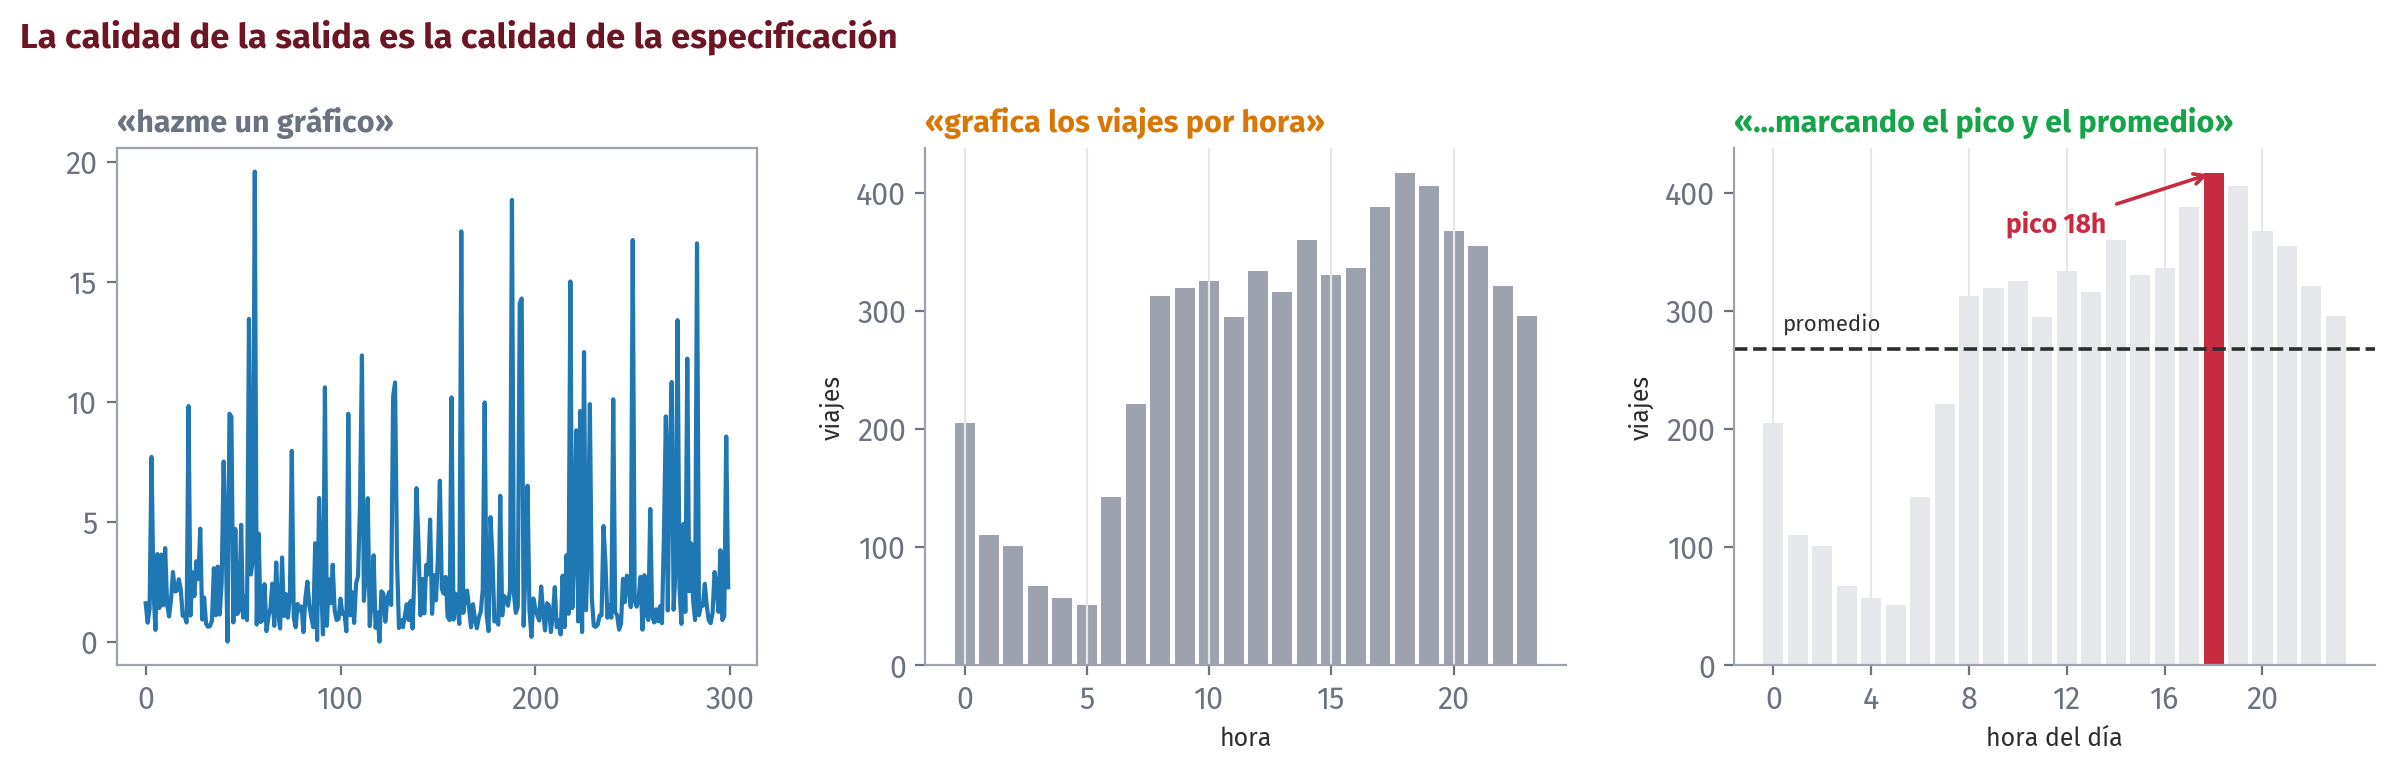
\includegraphics[width=0.97\textwidth, height=0.46\textheight, keepaspectratio]{fig_escalera_prompt.png}\end{center}
  \vspace{2pt}
  {\footnotesize\color{textMuted}
   El mismo agente, los mismos datos, tres pedidos distintos. \textbf{La
   calidad de la salida es la calidad de la especificación.}}
\end{frame}

\begin{frame}[shrink=6]{La Plantilla que se Llevan}
  \vspace{2pt}
  {\footnotesize\color{textMuted}
   Guárdenla. Sirve para pedir una gráfica, un análisis o una aplicación
   entera:}
  \vspace{6pt}
  \begin{prompt}[PLANTILLA GENERAL]
CONTEXTO: tengo [qué datos], con columnas [cuáles] en
[qué unidades]. Es para [quién / qué reunión].

OBJETIVO: quiero responder [qué pregunta].

RESTRICCIONES:
- usa [qué librerías]
- [qué NO hacer]
- en español, ejes con unidades

CRITERIO DE ACEPTACIÓN:
- [qué tiene que verse / cumplirse]
- avísame si [qué problema podría tener el dato]
  \end{prompt}
  \vspace{5pt}
  {\footnotesize\color{arcaDark}\bfseries
   Ese último renglón --- «avísame si...» --- es el que convierte al agente en
   un aliado para encontrar problemas, en vez de en alguien que los tapa.}
\end{frame}

\begin{frame}[shrink=8]{Segundo Encargo: Una Pregunta de Operación \hfill {\normalsize\color{arcaRed}\faClock\hspace{4pt}10 min}}
  \vspace{2pt}
  {\footnotesize\color{textMuted}
   Ahora una pregunta que un jefe de operaciones hace de verdad: \emph{¿cuándo
   conviene tener más gente en la calle?}}
  \vspace{6pt}
  \begin{prompt}[COPIAR Y PEGAR AL AGENTE]
CONTEXTO: el mismo DataFrame `taxis`. La columna
pickup tiene fecha y hora de inicio del viaje.

OBJETIVO: saber en qué combinaciones de día de la
semana y hora se concentra la demanda, para decidir
turnos.

RESTRICCIONES:
- un mapa de calor con seaborn (días en filas,
  horas en columnas)
- días en español y en orden lunes a domingo
- no uses colores rojo-verde (hay daltónicos
  en la sala)

CRITERIO DE ACEPTACIÓN:
- que se pueda señalar con el dedo el peor momento
- dime cuál es ese momento y cuántos viajes tiene
  \end{prompt}
\end{frame}

\begin{frame}[shrink=8]{Lo que Debería Salir}
  \vspace{-2pt}
  \begin{center}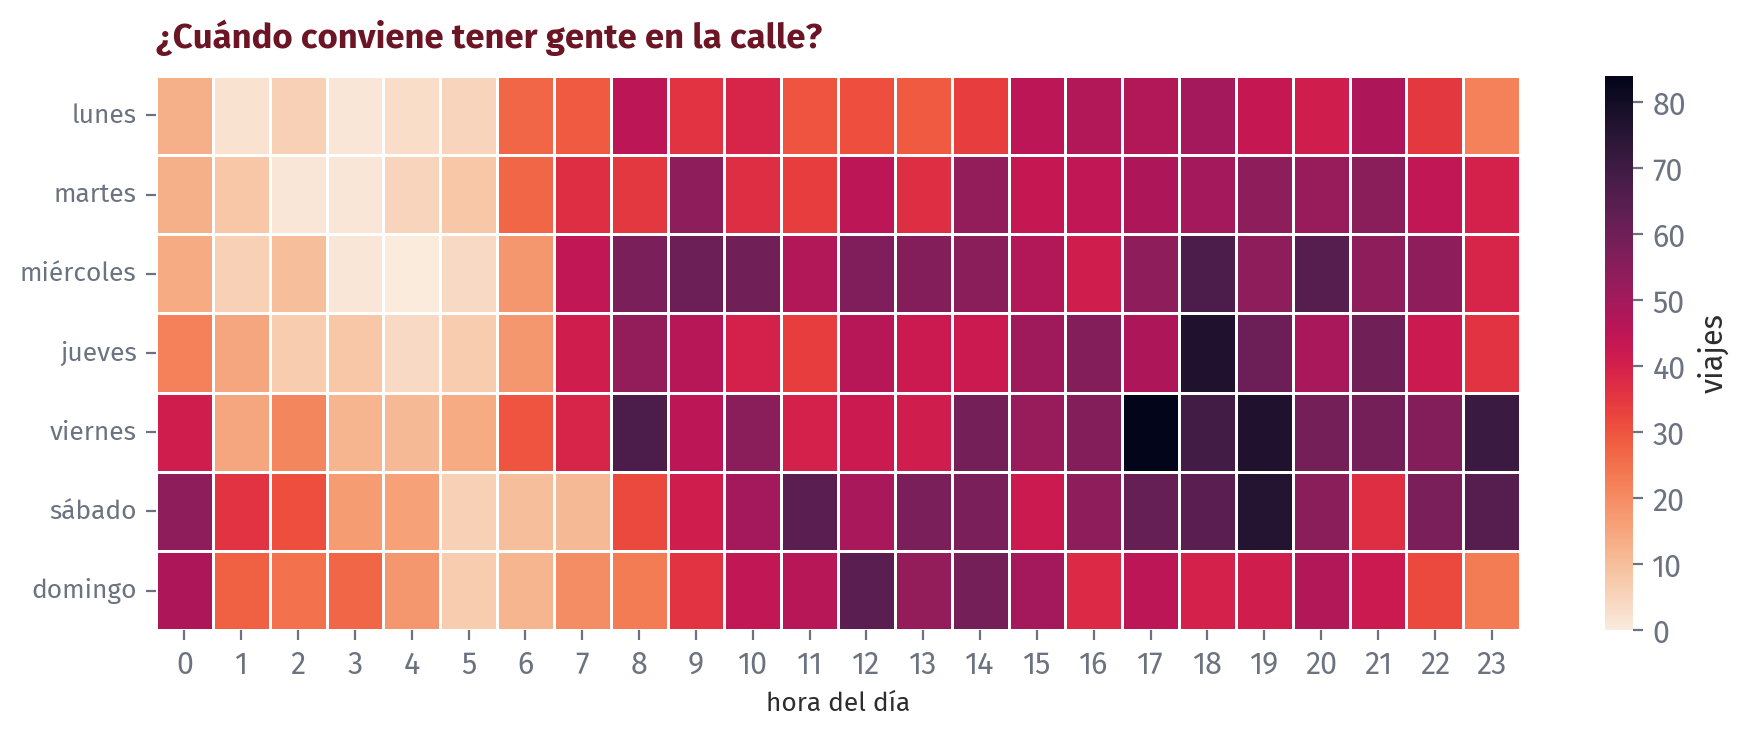
\includegraphics[width=0.97\textwidth, height=0.44\textheight, keepaspectratio]{fig_mapa_calor.png}\end{center}
  \vspace{2pt}
  {\footnotesize\color{textMuted}
   El momento de más demanda es el \textbf{viernes a las 17h}. Con eso ya se
   puede decidir un turno --- y esa decisión no la tomó el agente: la tomaron
   ustedes al preguntar bien.}
\end{frame}

% ═════════════════════════════════════════════════════════════════════════════
\sectionframe{Dónde Falla}{Y por qué sigue haciendo falta un ingeniero \\[6pt] \normalsize 70 -- 95 min}
% ═════════════════════════════════════════════════════════════════════════════

\begin{frame}[shrink=6]{Ahora la Parte Incómoda}
  \vspace{4pt}
  {\footnotesize\color{textMuted}
   Hasta acá todo salió bien, y esa es justamente la trampa. Un agente que
   funciona bien noventa veces genera confianza --- y a la vez noventa y uno
   hace algo que parece igual de bueno y está mal.
   \vspace{8pt}

   Vamos a hacer una pregunta perfectamente razonable sobre los mismos datos:}
  \vspace{7pt}
  \begin{tcolorbox}[colback=arcaGray, colframe=arcaDark, boxrule=0pt,
    leftrule=4pt, arc=3pt, left=10pt, right=10pt, top=7pt, bottom=7pt]
    {\footnotesize\color{arcaDark}\bfseries
     «¿Los pasajeros que pagan en efectivo dejan menos propina que los que
     pagan con tarjeta?»}\\[5pt]
    {\footnotesize\color{textMuted}
     Es el tipo de pregunta que se hace para decidir una política de medios de
     pago. Y tiene consecuencias reales en dinero.}
  \end{tcolorbox}
  \vspace{7pt}
  {\footnotesize\color{textMuted}\itshape
   El agente la responde en veinte segundos, con un gráfico impecable.}
\end{frame}

\begin{frame}[shrink=10]{Un Análisis Impecable}
  \vspace{-2pt}
  \begin{center}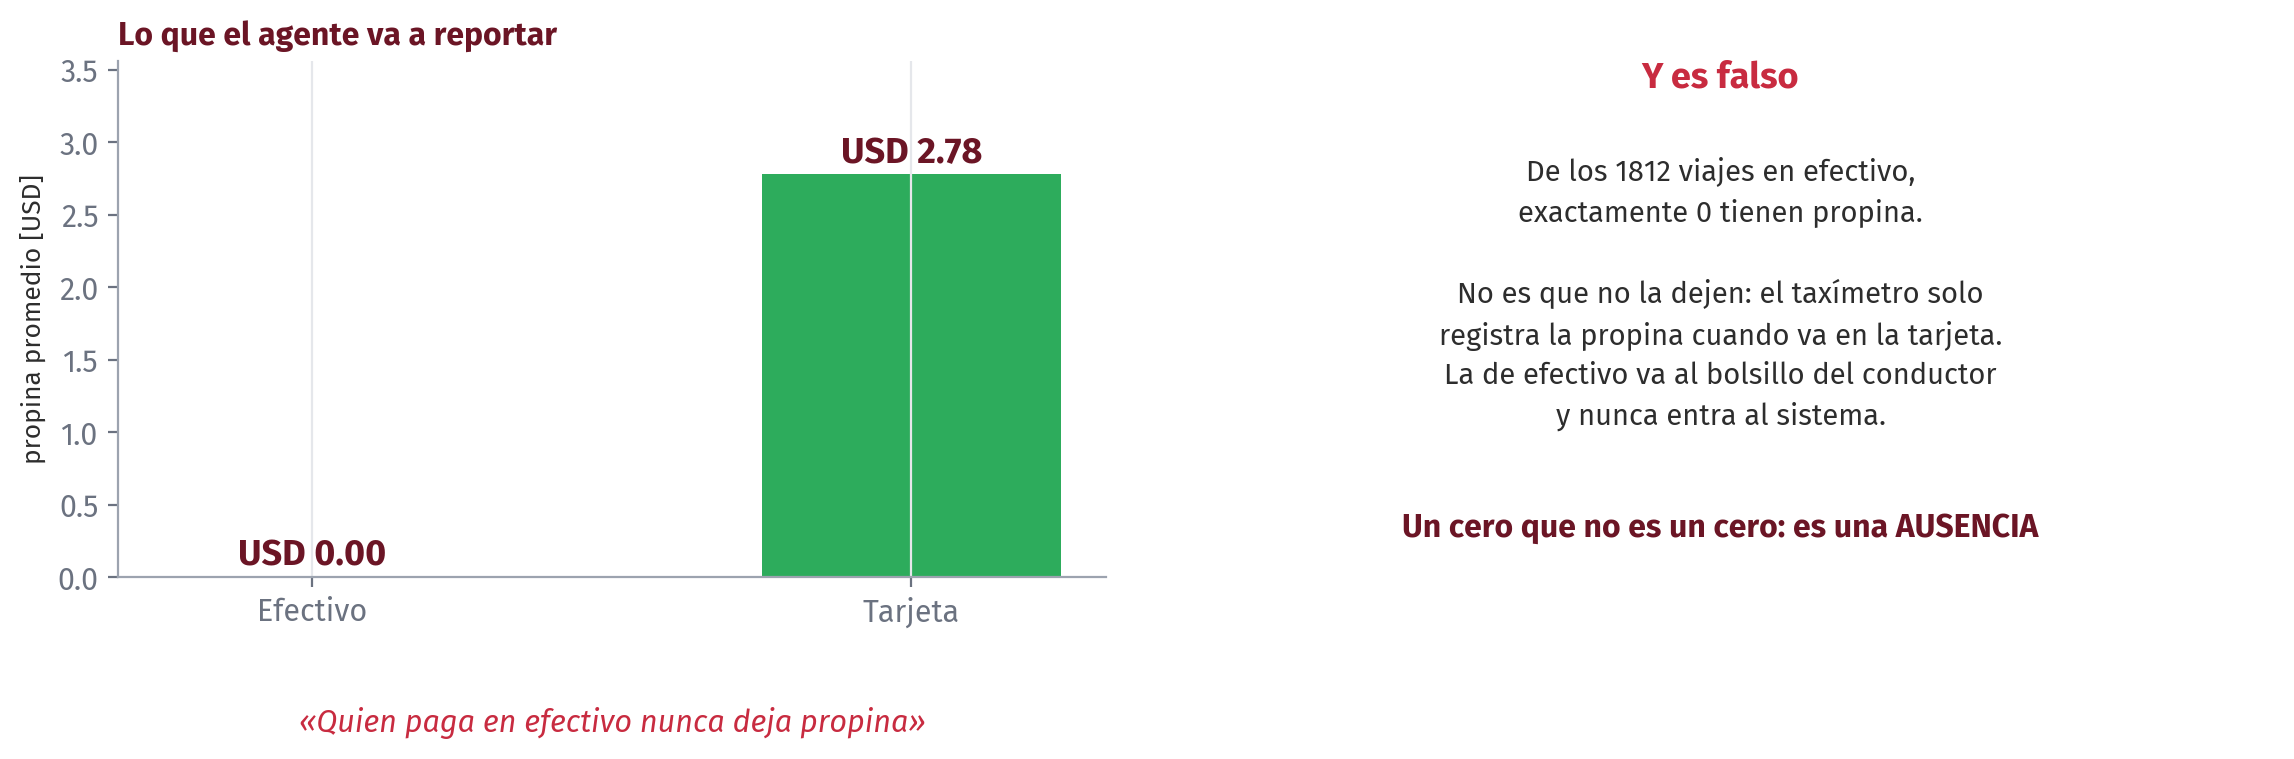
\includegraphics[width=0.97\textwidth, height=0.46\textheight, keepaspectratio]{fig_trampa.png}\end{center}
  \vspace{2pt}
  {\footnotesize\color{textMuted}
   El cálculo está bien hecho. El gráfico está bien hecho. La conclusión es
   \textbf{falsa}.}
\end{frame}

\begin{frame}[shrink=6]{Un Cero que No Es un Cero}
  \vspace{4pt}
  {\footnotesize\color{textMuted}
   De los \textbf{1.812} viajes pagados en efectivo, los que tienen propina
   registrada son \textbf{exactamente cero}. No 3, no 50: cero.
   \vspace{7pt}

   Ese número perfecto es la pista. En datos reales, nada es exactamente cero
   por casualidad.}
  \vspace{8pt}
  \begin{tcolorbox}[colback=arcaGray, colframe=arcaRed, boxrule=0pt,
    leftrule=4pt, arc=3pt, left=10pt, right=10pt, top=7pt, bottom=7pt]
    {\footnotesize\color{arcaDark}\bfseries
     El taxímetro solo registra la propina cuando va en la tarjeta.}\\[5pt]
    {\footnotesize\color{textMuted}
     La propina en efectivo va directo al bolsillo del conductor y nunca entra
     al sistema. La columna no dice «no dejó propina»: dice \textbf{«no
     tengo ese dato»}.}
  \end{tcolorbox}
  \vspace{8pt}
  {\footnotesize\color{arcaDark}\bfseries
   Y si alguien decide con eso --- por ejemplo, empujar el pago con tarjeta
   para «recuperar» propinas --- toma una decisión de negocio sobre una
   ausencia de datos.}
\end{frame}

\begin{frame}[shrink=6]{Esto Ya lo Vivieron}
  \vspace{4pt}
  {\footnotesize\color{textMuted}
   Es exactamente el mismo problema que encontramos en el módulo del agua:
   campos que aparecían con \textbf{cero agua producida} durante veinticinco
   años.
   \vspace{7pt}

   No es que no produjeran agua. Es que el regulador \textbf{no la empezó a
   exigir hasta el año 2000}. Un cero que era una ausencia.}
  \vspace{9pt}
  \begin{tcolorbox}[colback=arcaGray, colframe=arcaDark, boxrule=0pt,
    leftrule=4pt, arc=3pt, left=10pt, right=10pt, top=7pt, bottom=7pt]
    {\footnotesize\color{arcaDark}\bfseries
     Distinto dominio, distinto dato, distinto país --- el mismo error.}\\[5pt]
    {\footnotesize\color{textMuted}
     Y en los dos casos, lo que lo detectó no fue una técnica: fue alguien que
     conocía el negocio y dijo \emph{«esto no puede ser»}.}
  \end{tcolorbox}
  \vspace{7pt}
  {\footnotesize\color{arcaDark}\bfseries\itshape
   El agente no tiene esa alarma. Ustedes sí.}
\end{frame}

\begin{frame}[shrink=8]{Y Cuidado con la Sensación}
  \vspace{-2pt}
  \begin{center}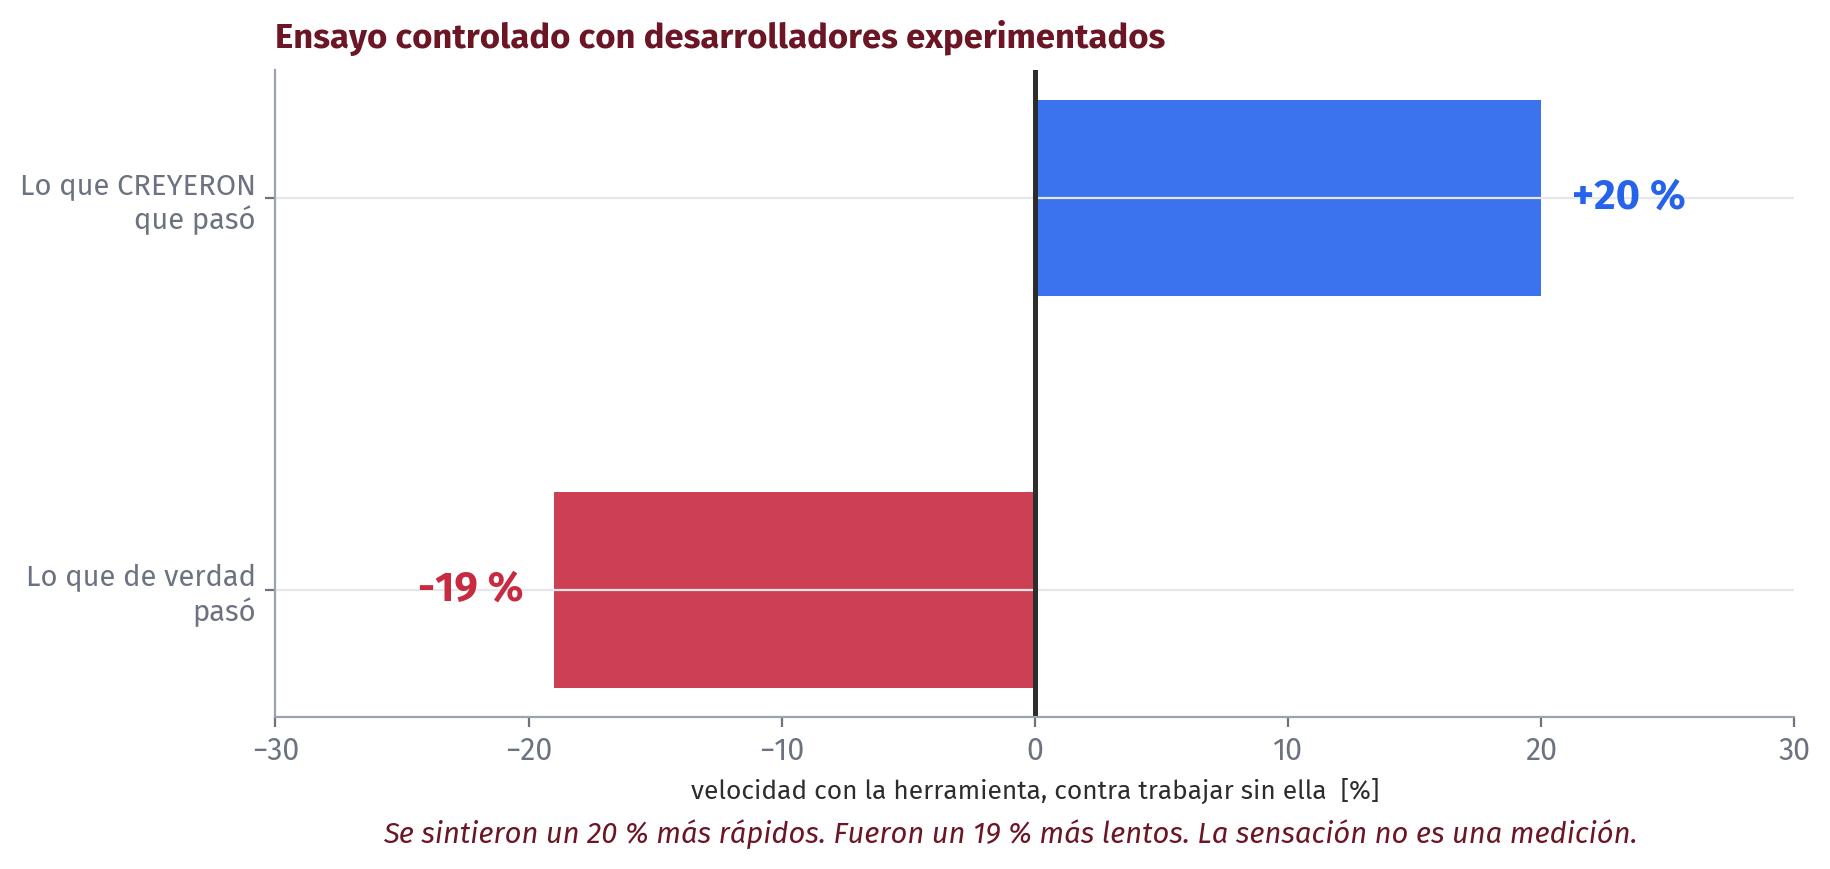
\includegraphics[width=0.88\textwidth, height=0.44\textheight, keepaspectratio]{fig_metr.png}\end{center}
  \vspace{2pt}
  {\footnotesize\color{textMuted}
   Un ensayo controlado con desarrolladores experimentados: se sintieron un
   \textbf{20\,\% más rápidos} y fueron un \textbf{19\,\% más lentos}. No es
   un argumento contra la herramienta --- es uno a favor de medir.}
\end{frame}

\begin{frame}[shrink=6]{La Lista de Verificación}
  \vspace{2pt}
  {\footnotesize\color{textMuted}
   Cuatro preguntas para cualquier resultado que devuelva un agente. Toman dos
   minutos y evitan la mayoría de los desastres:}
  \vspace{7pt}
  {\footnotesize\color{textMuted}
  \begin{enumerate}\setlength{\itemsep}{6pt}
    \item[{\color{arcaRed}\scriptsize\faSearch}]
      \textbf{¿Cuántas filas entraron y cuántas salieron?} Si el agente
      descartó la mitad de los datos sin avisar, todo lo demás sobra.
    \item[{\color{arcaRed}\scriptsize\faSearch}]
      \textbf{¿Hay ceros, vacíos o números redondos sospechosos?} Un cero
      perfecto casi siempre es una ausencia disfrazada.
    \item[{\color{arcaRed}\scriptsize\faSearch}]
      \textbf{¿El resultado tiene sentido físico o de negocio?} Si dice que un
      pozo produce más que el campo entero, no hace falta revisar el código.
    \item[{\color{arcaRed}\scriptsize\faSearch}]
      \textbf{¿Qué decisión se tomaría con esto, y qué pasa si está mal?}
      Si la respuesta es «nada grave», sigan. Si no, verifiquen a mano.
  \end{enumerate}}
  \vspace{7pt}
  {\footnotesize\color{arcaDark}\bfseries\itshape
   Ninguna de las cuatro exige saber programar. Las cuatro exigen saber del
   negocio.}
\end{frame}

\begin{frame}[shrink=8]{El Ciclo Real de Trabajo}
  \vspace{-2pt}
  \begin{center}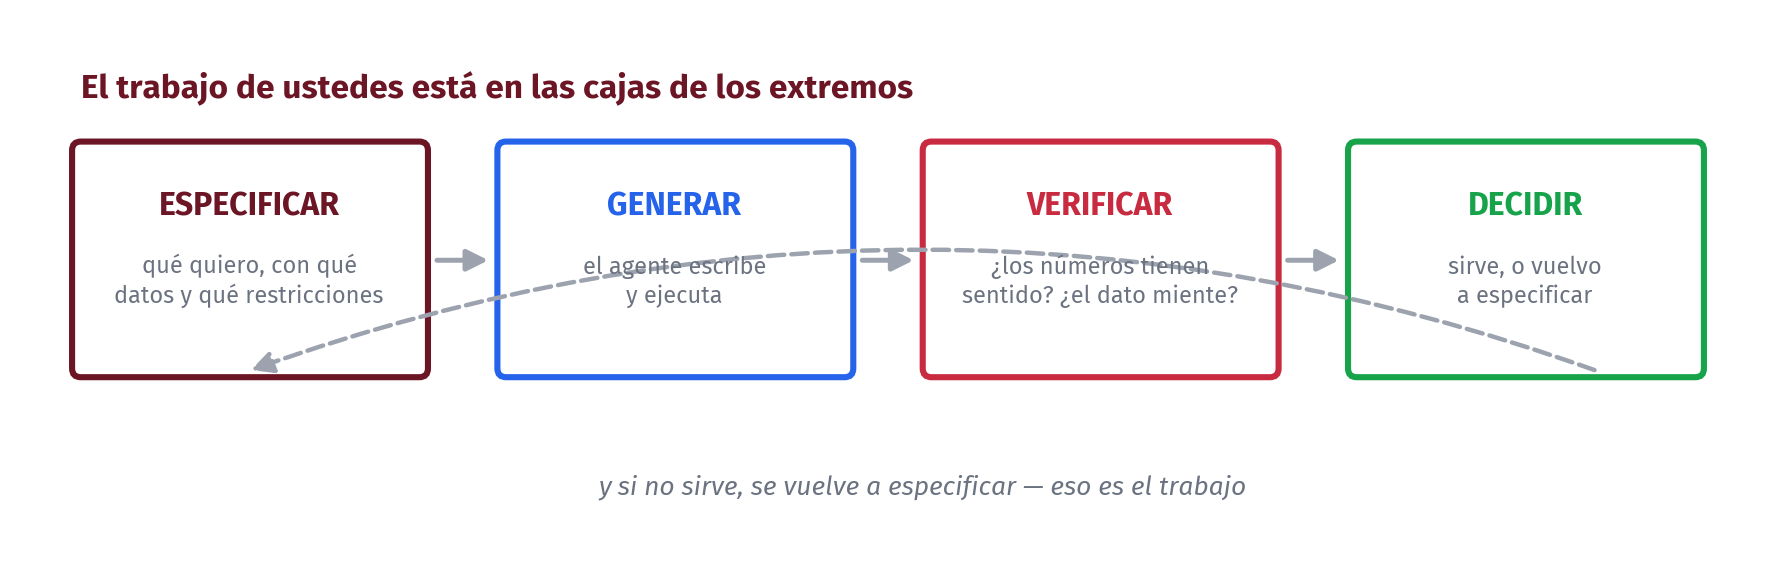
\includegraphics[width=0.97\textwidth, height=0.44\textheight, keepaspectratio]{fig_ciclo.png}\end{center}
  \vspace{2pt}
  {\footnotesize\color{textMuted}
   El agente hace la caja del medio. Las dos de los extremos --- especificar y
   decidir --- son de ustedes, y no se delegan.}
\end{frame}

\begin{frame}[shrink=6]{Tercer Encargo: Pónganle Trampas \hfill {\normalsize\color{arcaRed}\faClock\hspace{4pt}8 min}}
  \vspace{2pt}
  {\footnotesize\color{textMuted}
   Ahora usen al agente para lo contrario: para \textbf{buscar} problemas en
   vez de taparlos.}
  \vspace{6pt}
  \begin{prompt}[COPIAR Y PEGAR AL AGENTE]
CONTEXTO: DataFrame `taxis` de seaborn.

OBJETIVO: quiero saber si estos datos tienen algún
problema ANTES de sacar conclusiones.

Hazme una revisión de calidad que incluya:
- filas totales y filas con datos faltantes
- para cada columna numérica: mínimo, máximo, y
  cuántos valores son exactamente cero
- si alguna combinación de categorías tiene SIEMPRE
  el mismo valor (eso suele ser un artefacto del
  sistema que registra, no un hecho real)

CRITERIO DE ACEPTACIÓN:
- una tabla que yo pueda leer en 30 segundos
- y una lista de las cosas que te parecen raras,
  aunque no estés seguro
  \end{prompt}
  \vspace{3pt}
  {\scriptsize\color{arcaDark}\itshape
   Este prompt vale por toda la clase: guárdenlo y córranlo con cada dataset
   nuevo, antes de cualquier análisis.}
\end{frame}

% ═════════════════════════════════════════════════════════════════════════════
\sectionframe{De la Gráfica a la App}{Que otro lo pueda usar sin llamarlos \\[6pt] \normalsize 95 -- 120 min}
% ═════════════════════════════════════════════════════════════════════════════

\begin{frame}[shrink=8]{El Salto que Falta}
  \vspace{-2pt}
  \begin{center}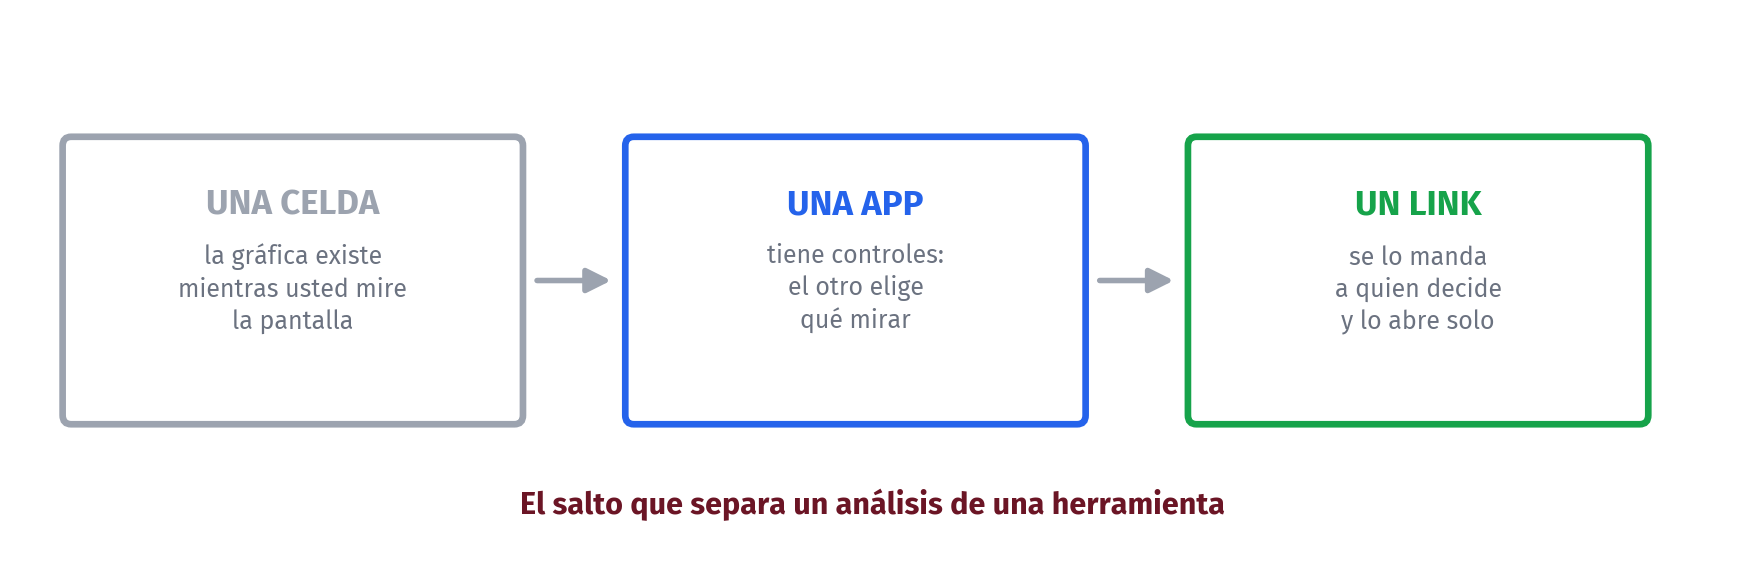
\includegraphics[width=0.95\textwidth, height=0.44\textheight, keepaspectratio]{fig_de_grafica_a_app.png}\end{center}
  \vspace{2pt}
  {\footnotesize\color{textMuted}
   Mientras el análisis viva en una celda, cada vez que alguien quiera ver
   otra cosa tiene que llamarlos. Una app se la mandan y se acabó.}
\end{frame}

\begin{frame}[shrink=6]{Qué Es Gradio}
  \vspace{4pt}
  {\footnotesize\color{textMuted}
   Una librería que convierte una función de Python en una página web con
   controles. Uno le dice: \emph{«esta función recibe una hora y devuelve un
   gráfico»}, y Gradio arma la interfaz sola.
   \vspace{8pt}

   No hay que saber nada de páginas web. Y en Colab hace algo muy útil: genera
   un \textbf{link público} que se le puede mandar a cualquiera.}
  \vspace{8pt}
  \begin{tcolorbox}[colback=arcaGray, colframe=arcaDark, boxrule=0pt,
    leftrule=3pt, arc=3pt, left=9pt, right=9pt, top=6pt, bottom=6pt]
    {\scriptsize\color{arcaDark}\bfseries LO QUE HAY QUE SABER DEL LINK}\\[4pt]
    {\footnotesize\color{textMuted}
     Funciona \textbf{mientras el cuaderno esté corriendo}. Si cierran Colab o
     se desconecta, el link deja de responder. Sirve perfecto para mostrar
     algo en una reunión; no sirve como sistema permanente.}
  \end{tcolorbox}
  \vspace{6pt}
  {\scriptsize\color{textMuted}\itshape
   Cómo se hace permanente lo vemos en la Clase 3. Hoy nos alcanza y sobra.}
\end{frame}

\begin{frame}[fragile, shrink=10]{La App Más Chica que Sirve}
  \vspace{2pt}
  \begin{minted}[fontsize=\scriptsize, breaklines]{python}
import gradio as gr

def ver_demanda(dia):
    d = taxis[taxis.dia_nombre == dia]
    return grafico_de_horas(d)

demo = gr.Interface(
    fn=ver_demanda,
    inputs=gr.Dropdown(DIAS, label="Día"),
    outputs=gr.Plot(label="Demanda por hora"),
    title="Demanda de taxis por día y hora")

demo.launch(share=True)
  \end{minted}
  \vspace{4pt}
  {\footnotesize\color{textMuted}
   Tres piezas: la \textbf{función} que hace el trabajo, los
   \textbf{controles} de entrada y salida, y \texttt{launch(share=True)} que
   publica el link.}
\end{frame}

\begin{frame}[shrink=8]{Su Turno: Construyan la Herramienta \hfill {\normalsize\color{arcaRed}\faClock\hspace{4pt}20 min}}
  \vspace{2pt}
  \begin{prompt}[COPIAR Y PEGAR AL AGENTE]
CONTEXTO: en este cuaderno ya tengo el DataFrame
`taxis` cargado y una función que grafica la demanda
por hora.

OBJETIVO: convertirlo en una app de Gradio que pueda
mandarle por link al jefe de operaciones.

La app tiene que dejarle elegir:
- el día de la semana
- el barrio de origen (pickup_borough)

y mostrarle el gráfico de demanda por hora para esa
combinación, más una línea de texto que diga cuál es
la hora pico y cuántos viajes tiene.

RESTRICCIONES:
- usa gradio, con launch(share=True)
- todo en español
- si la combinación elegida no tiene datos, que lo
  diga con un mensaje claro en vez de fallar

CRITERIO DE ACEPTACIÓN:
- me tiene que dar un link que yo pueda abrir
- y no se puede caer si elijo un barrio sin viajes
  \end{prompt}
\end{frame}

\begin{frame}[shrink=6]{El Entregable del Módulo}
  \vspace{2pt}
  {\footnotesize\color{textMuted}
   Empiecen a pensarlo desde hoy. En la última clase cada uno presenta:}
  \vspace{3pt}
  \begin{tcolorbox}[colback=arcaGray, colframe=codeGreen, boxrule=0pt,
    leftrule=4pt, arc=3pt, left=10pt, right=10pt, top=4pt, bottom=4pt]
    {\footnotesize\color{arcaDark}\bfseries
     Una aplicación que resuelva un problema real de su trabajo, construida
     dirigiendo a un agente, con su link funcionando.}
  \end{tcolorbox}
  \vspace{3pt}
  {\footnotesize\color{textMuted}
   Y con tres cosas más, que valen tanto como la app:
  \begin{itemize}\setlength{\itemsep}{3pt}
    \item[{\color{arcaRed}\scriptsize\faArrowRight}]
      \textbf{Los prompts que usaron.} Queremos ver cómo dirigieron, no solo
      qué salió.
    \item[{\color{arcaRed}\scriptsize\faArrowRight}]
      \textbf{Un error que el agente cometió}, y cómo lo detectaron.
    \item[{\color{arcaRed}\scriptsize\faArrowRight}]
      \textbf{Qué decisión se toma} con la herramienta, y quién la toma.
  \end{itemize}}
  \vspace{3pt}
  {\footnotesize\color{arcaDark}\bfseries\itshape
   Traigan su propio dato. Si no pueden por confidencialidad, lo hablamos ---
   hay maneras, y son parte de la Clase 3.}
\end{frame}

% ═════════════════════════════════════════════════════════════════════════════
\sectionframe{Cierre}{}
% ═════════════════════════════════════════════════════════════════════════════

\begin{frame}[shrink=8]{Lo Que Aprendimos Hoy}
  \vspace{-2pt}
  \begin{columns}[T]
    \begin{column}{0.48\textwidth}
      {\small\color{arcaDark}\bfseries\faLightbulb[regular]\hspace{5pt}Conceptos:}
      \vspace{4pt}
      {\footnotesize\color{textMuted}
      \begin{itemize}\setlength{\itemsep}{3pt}
        \item[{\color{codeGreen}\scriptsize\faCheck}]
          Autocompletado, asistente y \textbf{agente} no son lo mismo
        \item[{\color{codeGreen}\scriptsize\faCheck}]
          Una gráfica es un \textbf{argumento}, no un adorno
        \item[{\color{codeGreen}\scriptsize\faCheck}]
          Los \textbf{cuatro fundamentos}: objetivo, contexto,
          restricciones, criterio de aceptación
        \item[{\color{codeGreen}\scriptsize\faCheck}]
          Un \textbf{cero perfecto} casi siempre es una ausencia
        \item[{\color{codeGreen}\scriptsize\faCheck}]
          La \textbf{lista de verificación} de cuatro preguntas
      \end{itemize}}
    \end{column}
    \begin{column}{0.48\textwidth}
      {\small\color{arcaDark}\bfseries\faTools\hspace{5pt}Herramientas:}
      \vspace{4pt}
      {\footnotesize\color{textMuted}
      \begin{itemize}\setlength{\itemsep}{3pt}
        \item[{\color{arcaRed}\scriptsize\faArrowRight}]
          \texttt{seaborn} y \texttt{load\_dataset}
        \item[{\color{arcaRed}\scriptsize\faArrowRight}]
          El panel de Gemini de Colab
        \item[{\color{arcaRed}\scriptsize\faArrowRight}]
          \texttt{gradio} y \texttt{launch(share=True)}
        \item[{\color{arcaRed}\scriptsize\faArrowRight}]
          La \textbf{plantilla de prompt} --- la que más van a usar
      \end{itemize}}
      \vspace{6pt}
      \begin{tcolorbox}[colback=arcaGray, colframe=arcaRed, boxrule=0pt, leftrule=3pt,
        arc=3pt, left=6pt, right=6pt, top=4pt, bottom=4pt]
        {\scriptsize\color{arcaRed}\bfseries EL NÚMERO DEL DÍA}\\[3pt]
        {\scriptsize\color{textMuted}
         \textbf{1.812 y 0.} Los viajes en efectivo, y los que tenían propina
         registrada. El agente no vio nada raro.}
      \end{tcolorbox}
    \end{column}
  \end{columns}
\end{frame}

\begin{frame}[shrink=6]{El Resultado Negativo de Hoy}
  \vspace{4pt}
  {\footnotesize\color{textMuted}
   La regla de este curso es que al menos un resultado negativo se dice en voz
   alta. Hoy hubo dos, y los dos están medidos:}
  \vspace{7pt}
  {\footnotesize\color{textMuted}
  \begin{enumerate}\setlength{\itemsep}{7pt}
    \item[{\color{arcaRed}\scriptsize\faTimes}]
      \textbf{El agente entregó un análisis correcto con una conclusión
      falsa}, y no dio ninguna señal de alarma. El código estaba bien; el dato
      mentía.
    \item[{\color{arcaRed}\scriptsize\faTimes}]
      \textbf{En un ensayo controlado, desarrolladores experimentados fueron
      19\,\% más lentos} usando estas herramientas, mientras se sentían 20\,\%
      más rápidos.
  \end{enumerate}}
  \vspace{8pt}
  \begin{tcolorbox}[colback=arcaGray, colframe=arcaDark, boxrule=0pt,
    leftrule=4pt, arc=3pt, left=10pt, right=10pt, top=7pt, bottom=7pt]
    {\footnotesize\color{arcaDark}\bfseries
     Ninguno de los dos es razón para no usarlas. Los dos son razón para
     \textbf{medir en vez de confiar en la sensación} --- que es exactamente
     lo que venimos haciendo todo el diplomado.}
  \end{tcolorbox}
\end{frame}

\begin{frame}[shrink=6]{Si Se Llevan Una Sola Cosa}
  \vspace{6pt}
  \begin{tcolorbox}[colback=arcaGray, colframe=arcaRed, boxrule=0pt, leftrule=4pt,
    arc=3pt, left=10pt, right=10pt, top=9pt, bottom=9pt]
    {\large\color{arcaDark}\bfseries
     El agente escribe el código. Ustedes responden por el resultado.}\\[7pt]
    {\footnotesize\color{textMuted}
     Y eso no es una carga: es la razón por la que su criterio vale más ahora
     que hace tres años. Escribir se volvió barato; saber si el resultado
     tiene sentido, no.\\[6pt]
     La habilidad que se llevan hoy no es «usar Gemini». Es
     \textbf{especificar bien y verificar siempre} --- y eso sirve con
     cualquier herramienta que salga el año que viene.}
  \end{tcolorbox}
  \vspace{8pt}
  {\footnotesize\color{arcaDark}\itshape
   Nadie en esta sala escribió una línea de código hoy. Y todos se van con una
   aplicación funcionando.}
\end{frame}

\begin{frame}[shrink=6]{Lo Que Sigue}
  \vspace{4pt}
  {\footnotesize\color{textMuted}
  \begin{itemize}\setlength{\itemsep}{7pt}
    \item[{\color{arcaRed}\faArrowCircleRight}]
      \textbf{Clase 2 --- Que responda, y que no mienta.} Cómo se sirve un
      modelo de verdad: qué entra, qué sale, qué pasa cuando le mandan un dato
      raro. Y el error más caro de todos: el que funciona en el cuaderno y
      falla en producción.
    \item[{\color{arcaRed}\faArrowCircleRight}]
      \textbf{Clase 3 --- Los peligros, con nombre y apellido.}
      Confidencialidad --- qué se puede pegar en un chat de IA y qué no ---,
      librerías que el agente inventa, y código que corre y está mal.
    \item[{\color{arcaRed}\faArrowCircleRight}]
      \textbf{Clase 4 --- Su proyecto.} Cada uno con su problema y su
      herramienta, presentada al grupo.
  \end{itemize}}
  \vspace{8pt}
  \begin{tcolorbox}[colback=arcaGray, colframe=codeGreen, boxrule=0pt, leftrule=3pt,
    arc=3pt, left=8pt, right=8pt, top=5pt, bottom=5pt]
    {\scriptsize\color{codeGreen}\bfseries\faCheck\hspace{4pt}TAREA PARA LA PRÓXIMA}\\[4pt]
    {\scriptsize\color{textMuted}
     Piensen en \textbf{un} problema de su trabajo donde hoy alguien pierde
     tiempo con una hoja de cálculo. Ese es su proyecto. Tráiganlo escrito en
     dos frases.}
  \end{tcolorbox}
\end{frame}

\begin{frame}[shrink=8]{Datos y Referencias}
  \vspace{4pt}
  {\footnotesize\color{textMuted}
  \begin{itemize}\setlength{\itemsep}{5pt}
    \item[{\color{arcaRed}\scriptsize\faChartBar}]
      \textbf{Adopción y confianza:} Stack Overflow Developer Survey y su
      análisis de la brecha de confianza (2026); \emph{State of Code}, Sonar
      (enero de 2026).
    \item[{\color{arcaRed}\scriptsize\faChartBar}]
      \textbf{Productividad medida:} ensayo controlado de \textbf{METR} con
      desarrolladores experimentados; informes de adopción de agentes 2026.
    \item[{\color{arcaRed}\scriptsize\faDatabase}]
      \textbf{Datos:} \texttt{taxis}, \texttt{healthexp} y \texttt{flights},
      de los conjuntos de práctica que trae \textbf{seaborn}. Se cargan con
      una línea y no hay que bajar nada.
    \item[{\color{arcaRed}\scriptsize\faFileCode}]
      Las figuras y \textbf{todas} las cifras de estas láminas salen de
      \texttt{figuras.py}. Nada está escrito a mano.
  \end{itemize}}
  \vspace{7pt}
  {\scriptsize\color{arcaDark}\itshape
   Como siempre: corren el script y tiene que dar exactamente lo mismo. Si no
   da, es un error nuestro y queremos saberlo.}
\end{frame}

% ── GRACIAS ──────────────────────────────────────────────────────────────────
\begingroup
\setbeamertemplate{headline}{}
\setbeamertemplate{footline}{}
\setbeamertemplate{navigation symbols}{}
\begin{frame}[plain, noframenumbering]
  \begin{tikzpicture}[remember picture, overlay]
    \fill[arcaDark] (current page.south west) rectangle (current page.north east);
    \node[anchor=center, text=white, font=\Huge\bfseries]
      at ([yshift=1.5cm]current page.center) {¡Gracias!};
    \node[anchor=center, text=white!80, font=\large, text width=10cm, align=center]
      at ([yshift=0.2cm]current page.center)
      {Carlos Enrique Mosquera Trujillo};
    \node[anchor=center, text=white!60, font=\normalsize, text width=10cm, align=center]
      at ([yshift=-0.6cm]current page.center)
      {\faEnvelope\hspace{6pt}cmosquerat@unal.edu.co};
    \node[anchor=center, text=white!60, font=\normalsize, text width=11cm, align=center]
      at ([yshift=-1.3cm]current page.center)
      {Machine Learning for Petroleum Engineers Using Python};
    \node[anchor=center, text=white!40, font=\small]
      at ([yshift=-2.0cm]current page.center)
      {Módulo 7 · Clase 1 \quad$\cdot$\quad SLB Ecuador \quad$\cdot$\quad UDLA \quad$\cdot$\quad 2026};
  \end{tikzpicture}
\end{frame}
\endgroup

\end{document}
